\documentclass[aspectratio=169, serif]{beamer}
% \usepackage[T1]{fontenc} % Needed for Type1 Concrete
% \usepackage[charter]{mathdesign}
\usetheme{metropolis}

\usepackage{neuralnetwork}
\usepackage{tikz, ifthen}
\usetikzlibrary{positioning}

\renewcommand{\thefootnote}{\alph{footnote}}

\pagestyle{empty}

\usepackage{kotex}
\usepackage{booktabs}
\usepackage{nicematrix}

\usepackage{amsmath}
\usepackage{amsfonts}
\usepackage{amssymb}
\usepackage{graphicx}
\usepackage{tabularx}

\usepackage{caption}
\usepackage{subcaption}

\captionsetup[subfigure]{labelformat=empty}

\usepackage[
backend=biber,
style=authoryear-icomp,
maxbibnames=9,maxcitenames=2,
sorting=nty
]{biblatex}
\addbibresource{literature.bib}

\title{Reconstruction of Coronal Magnetic Fields \\ using Physics-Informed Neural Networks}

\date{}
\author{전민규}
\institute{학사졸업논문}

\begin{document}
  \maketitle

  \begin{frame}{The 3D magnetic fields}
    \begin{columns}
        \begin{column}{0.9\textwidth}
        \begin{figure}
            \only<1>{
            \begin{subfigure}{.5\linewidth}
              \centering
              \caption{\large PINN(0)}
              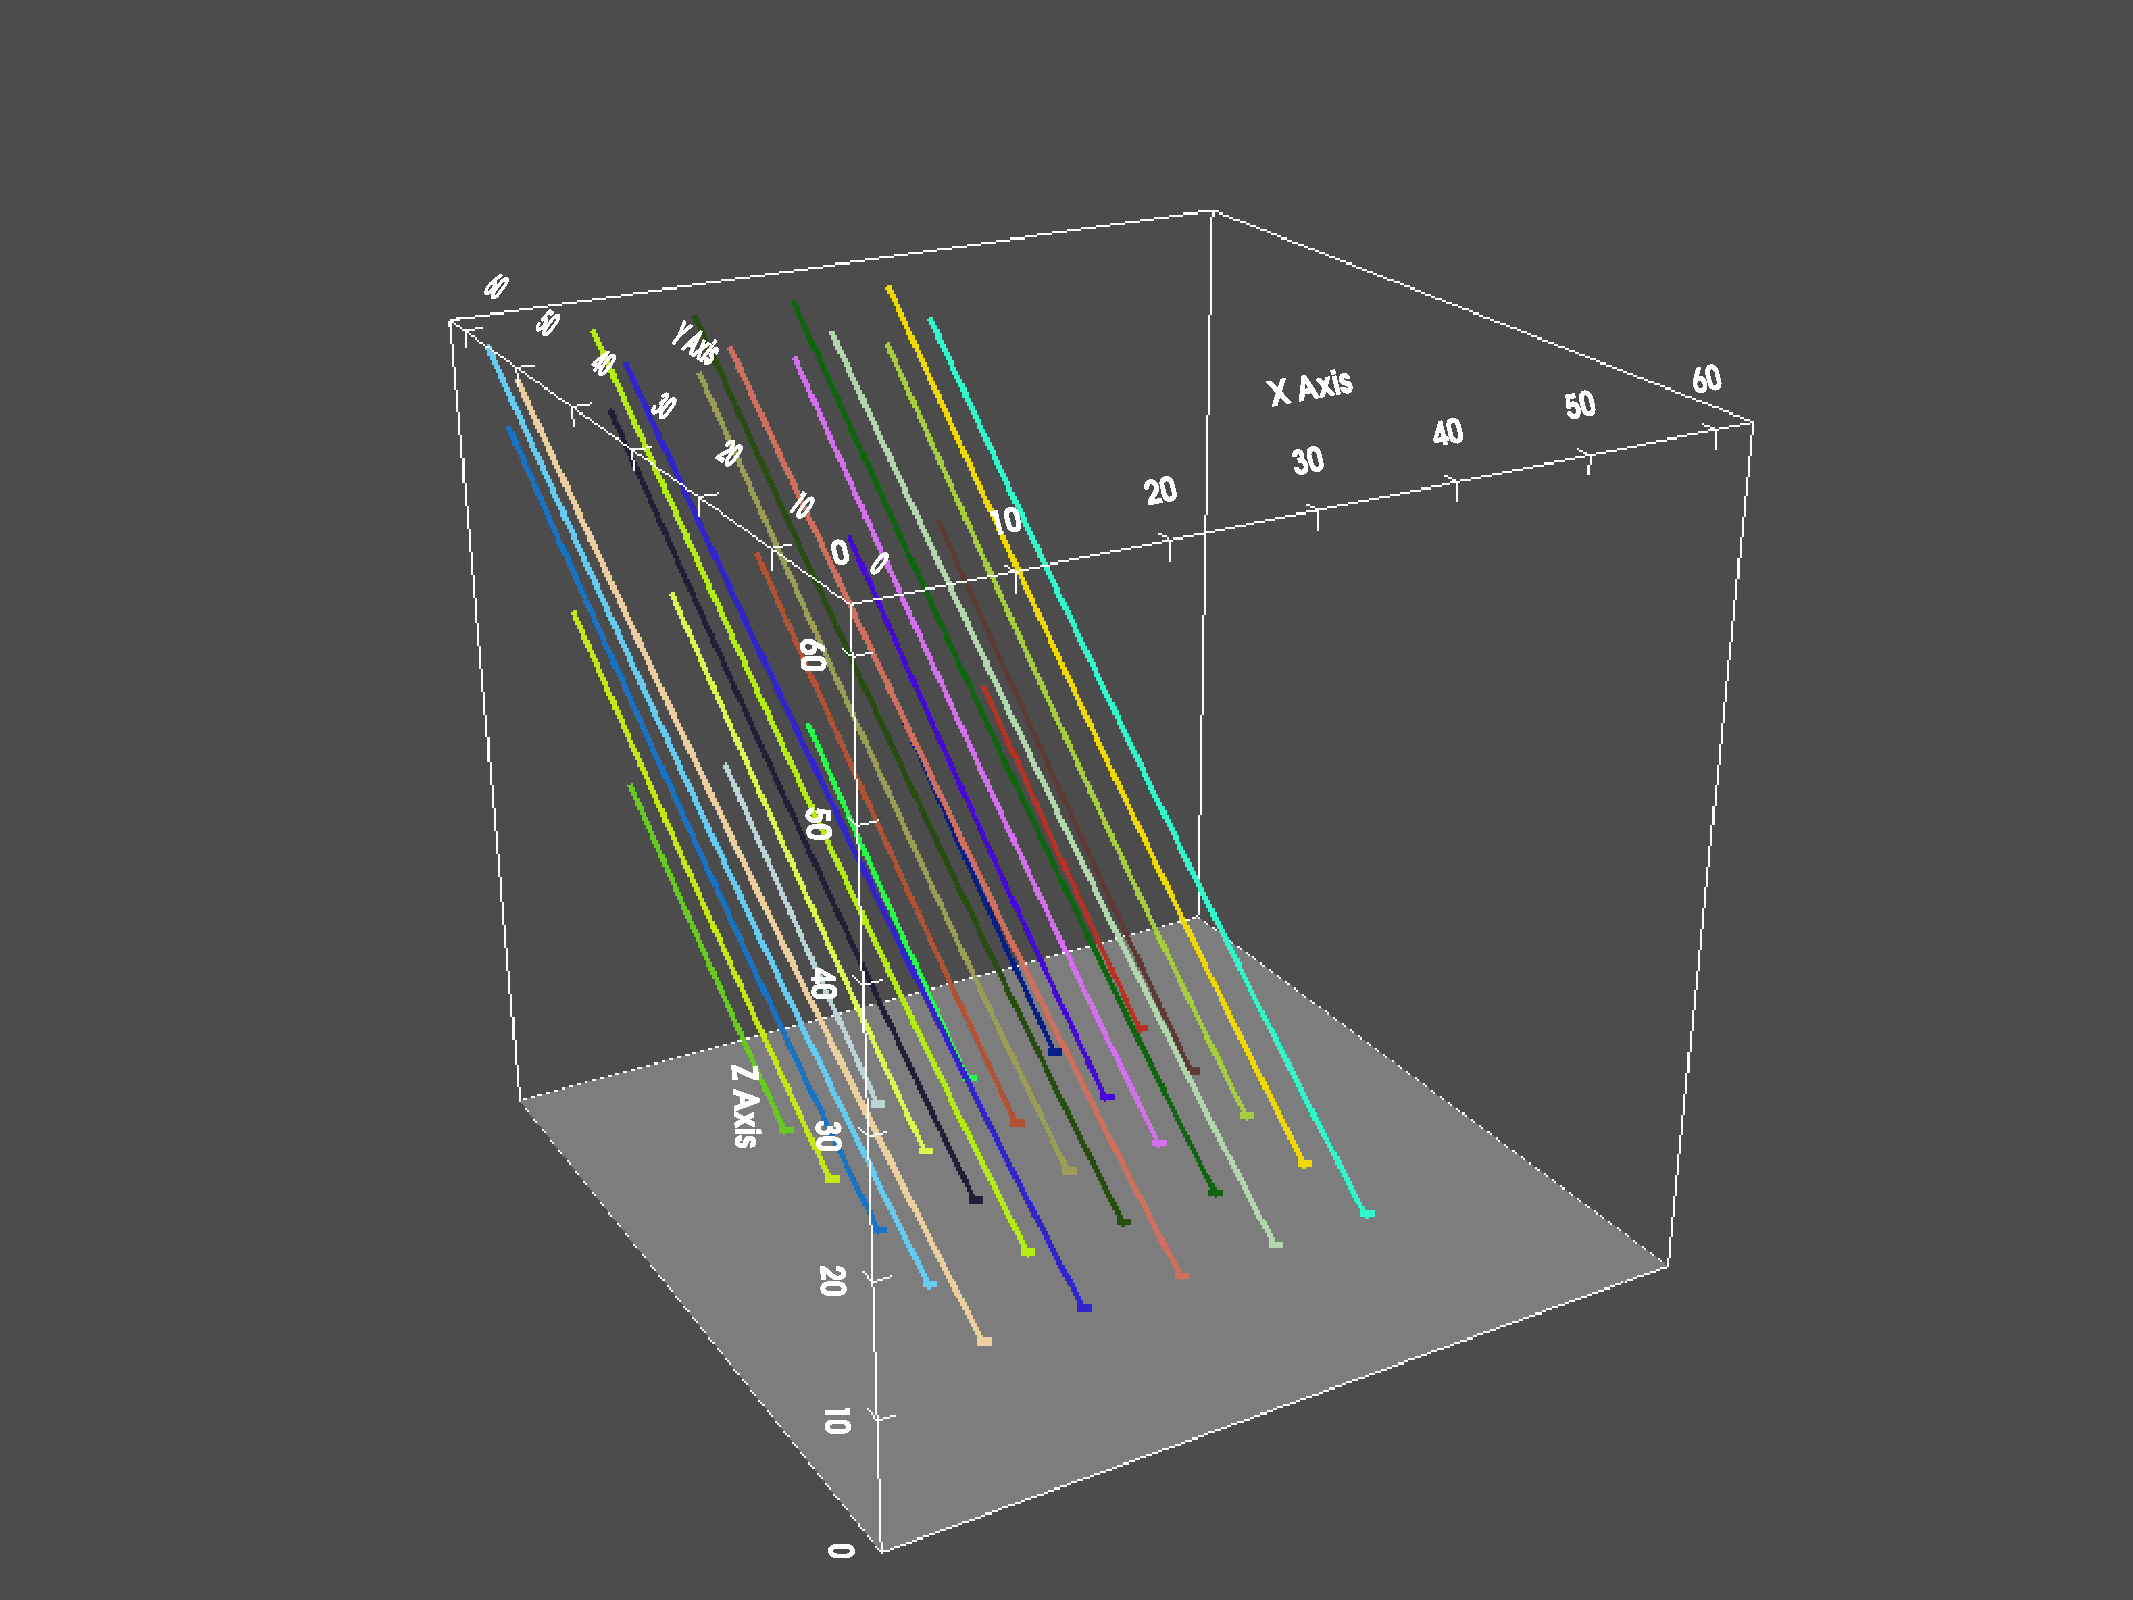
\includegraphics[trim={6cm 0cm 6cm 3cm}, clip, width=\linewidth]{"../../Thesis/img/PINN_000000_xz_tilted.pdf"}
            \end{subfigure}%
            \begin{subfigure}{.5\linewidth}
                \centering
                \caption{\large Low-Lou}
                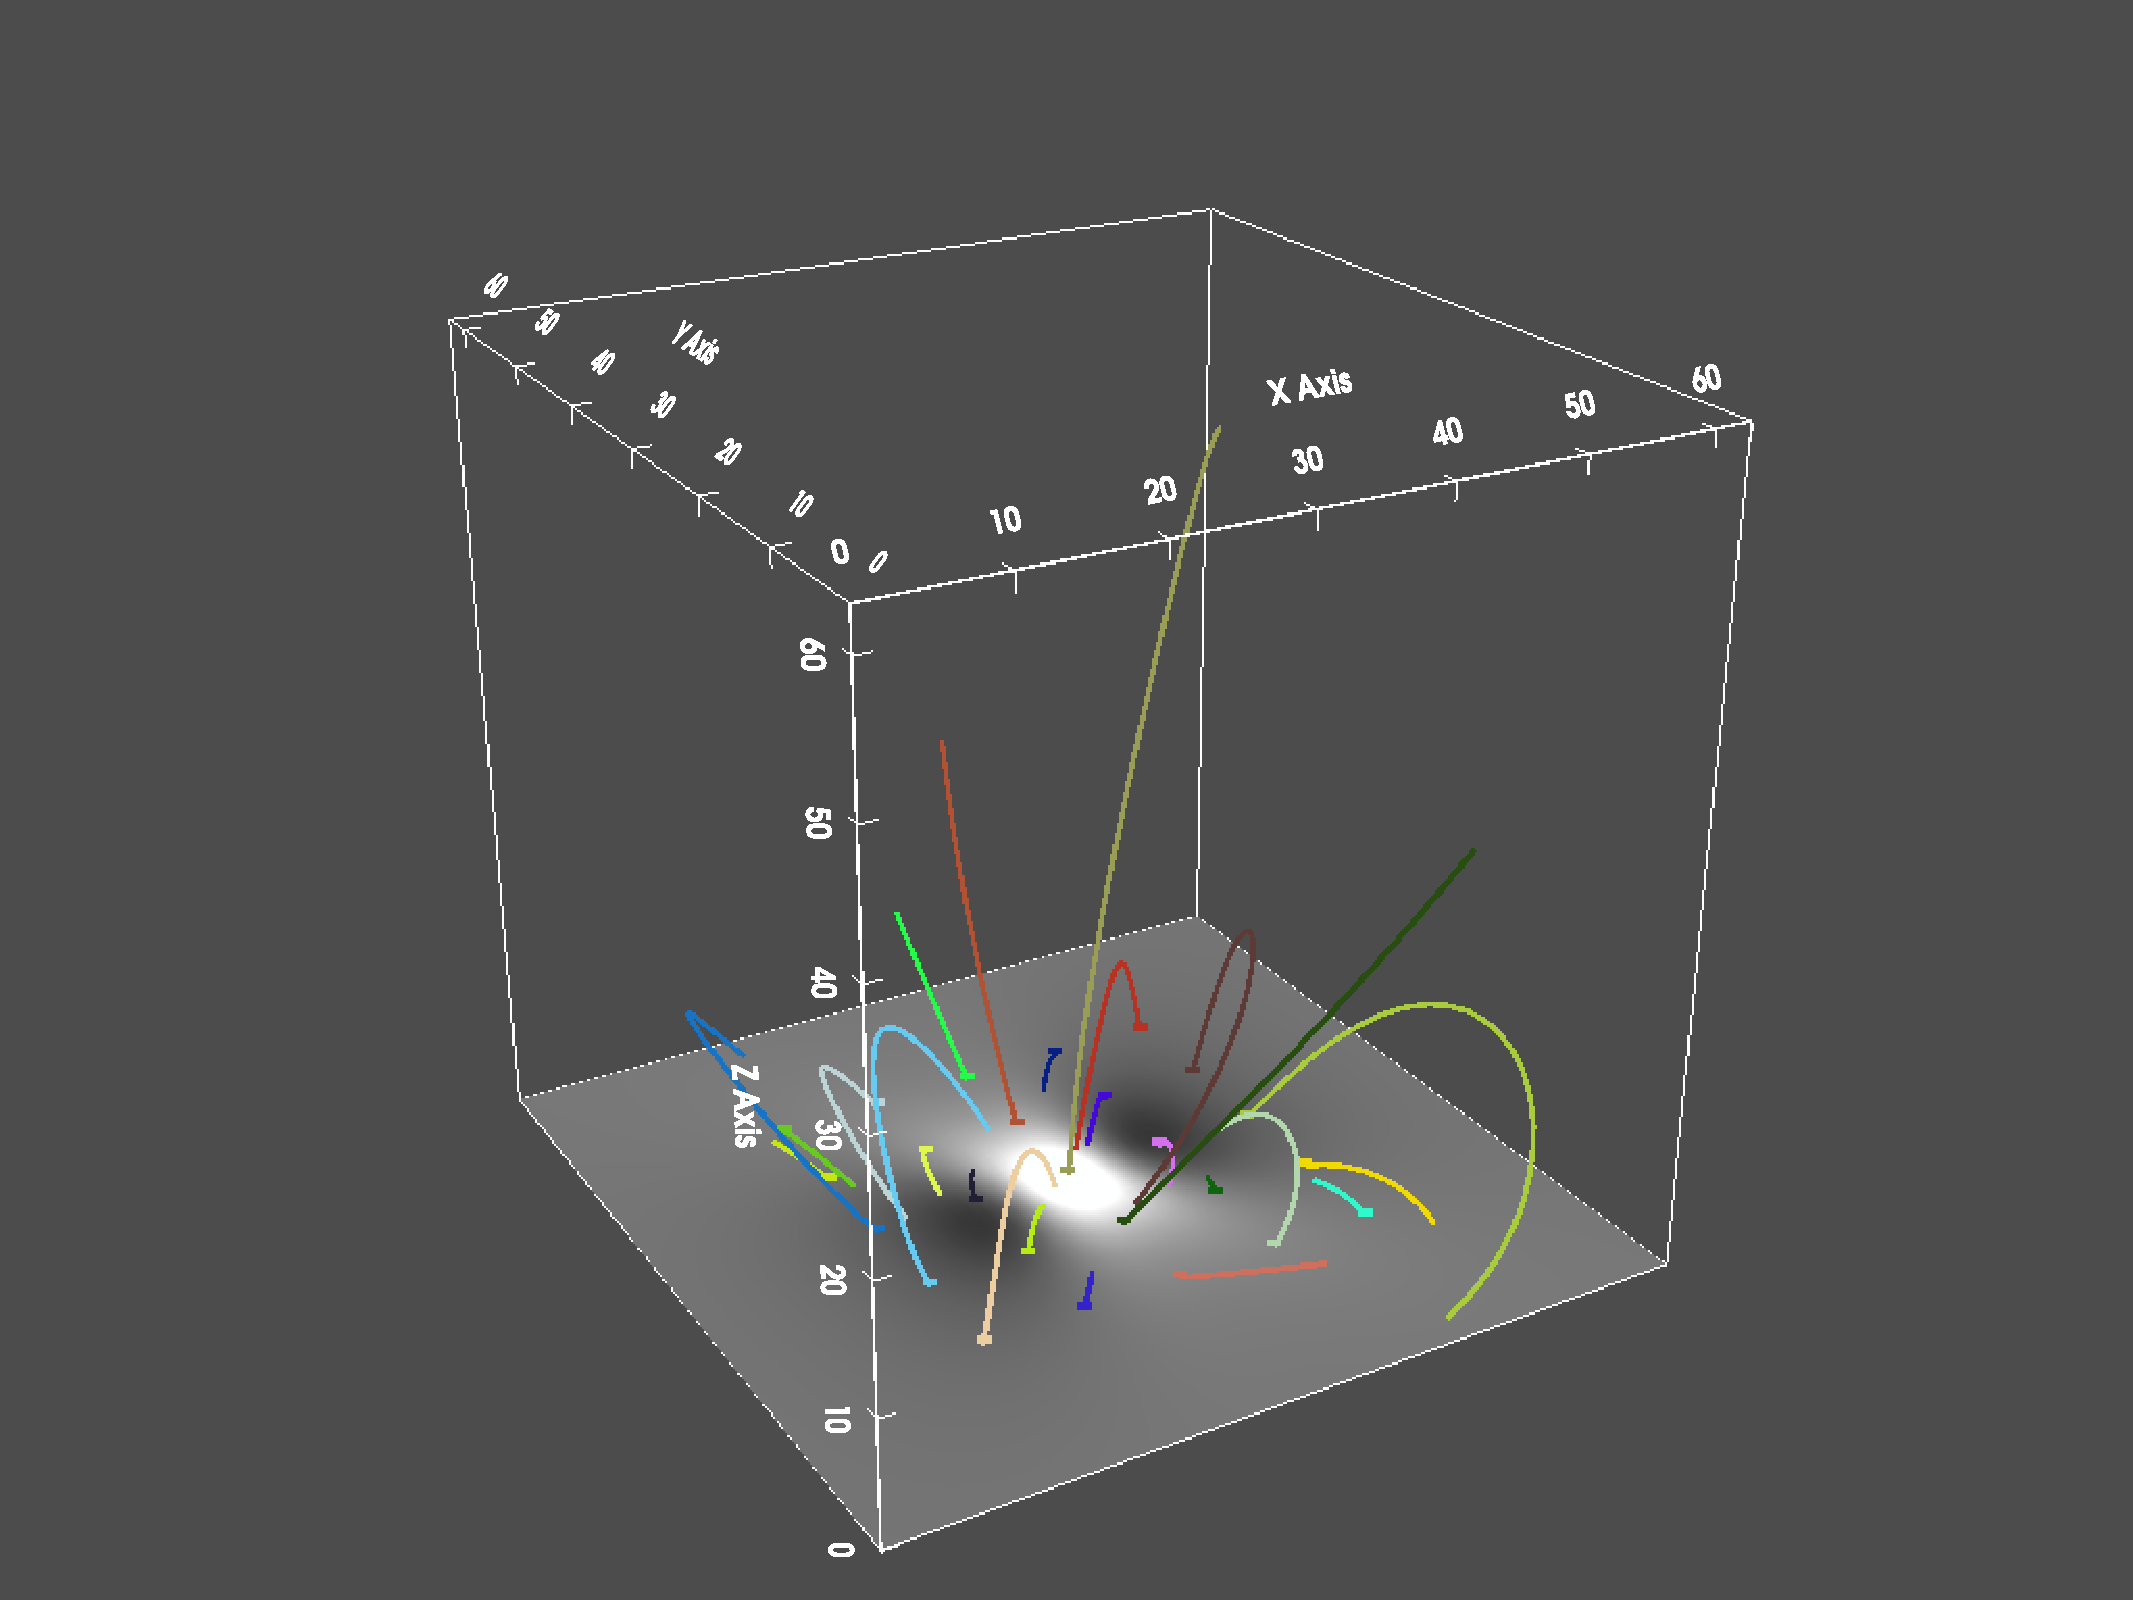
\includegraphics[trim={6cm 0cm 6cm 3cm}, clip, width=\linewidth]{"../../Thesis/img/LL_xz_tilted.pdf"}
              \end{subfigure}
            }

            \only<2>{
            \begin{subfigure}{.5\linewidth}
              \centering
              \caption{\large PINN(100)}
              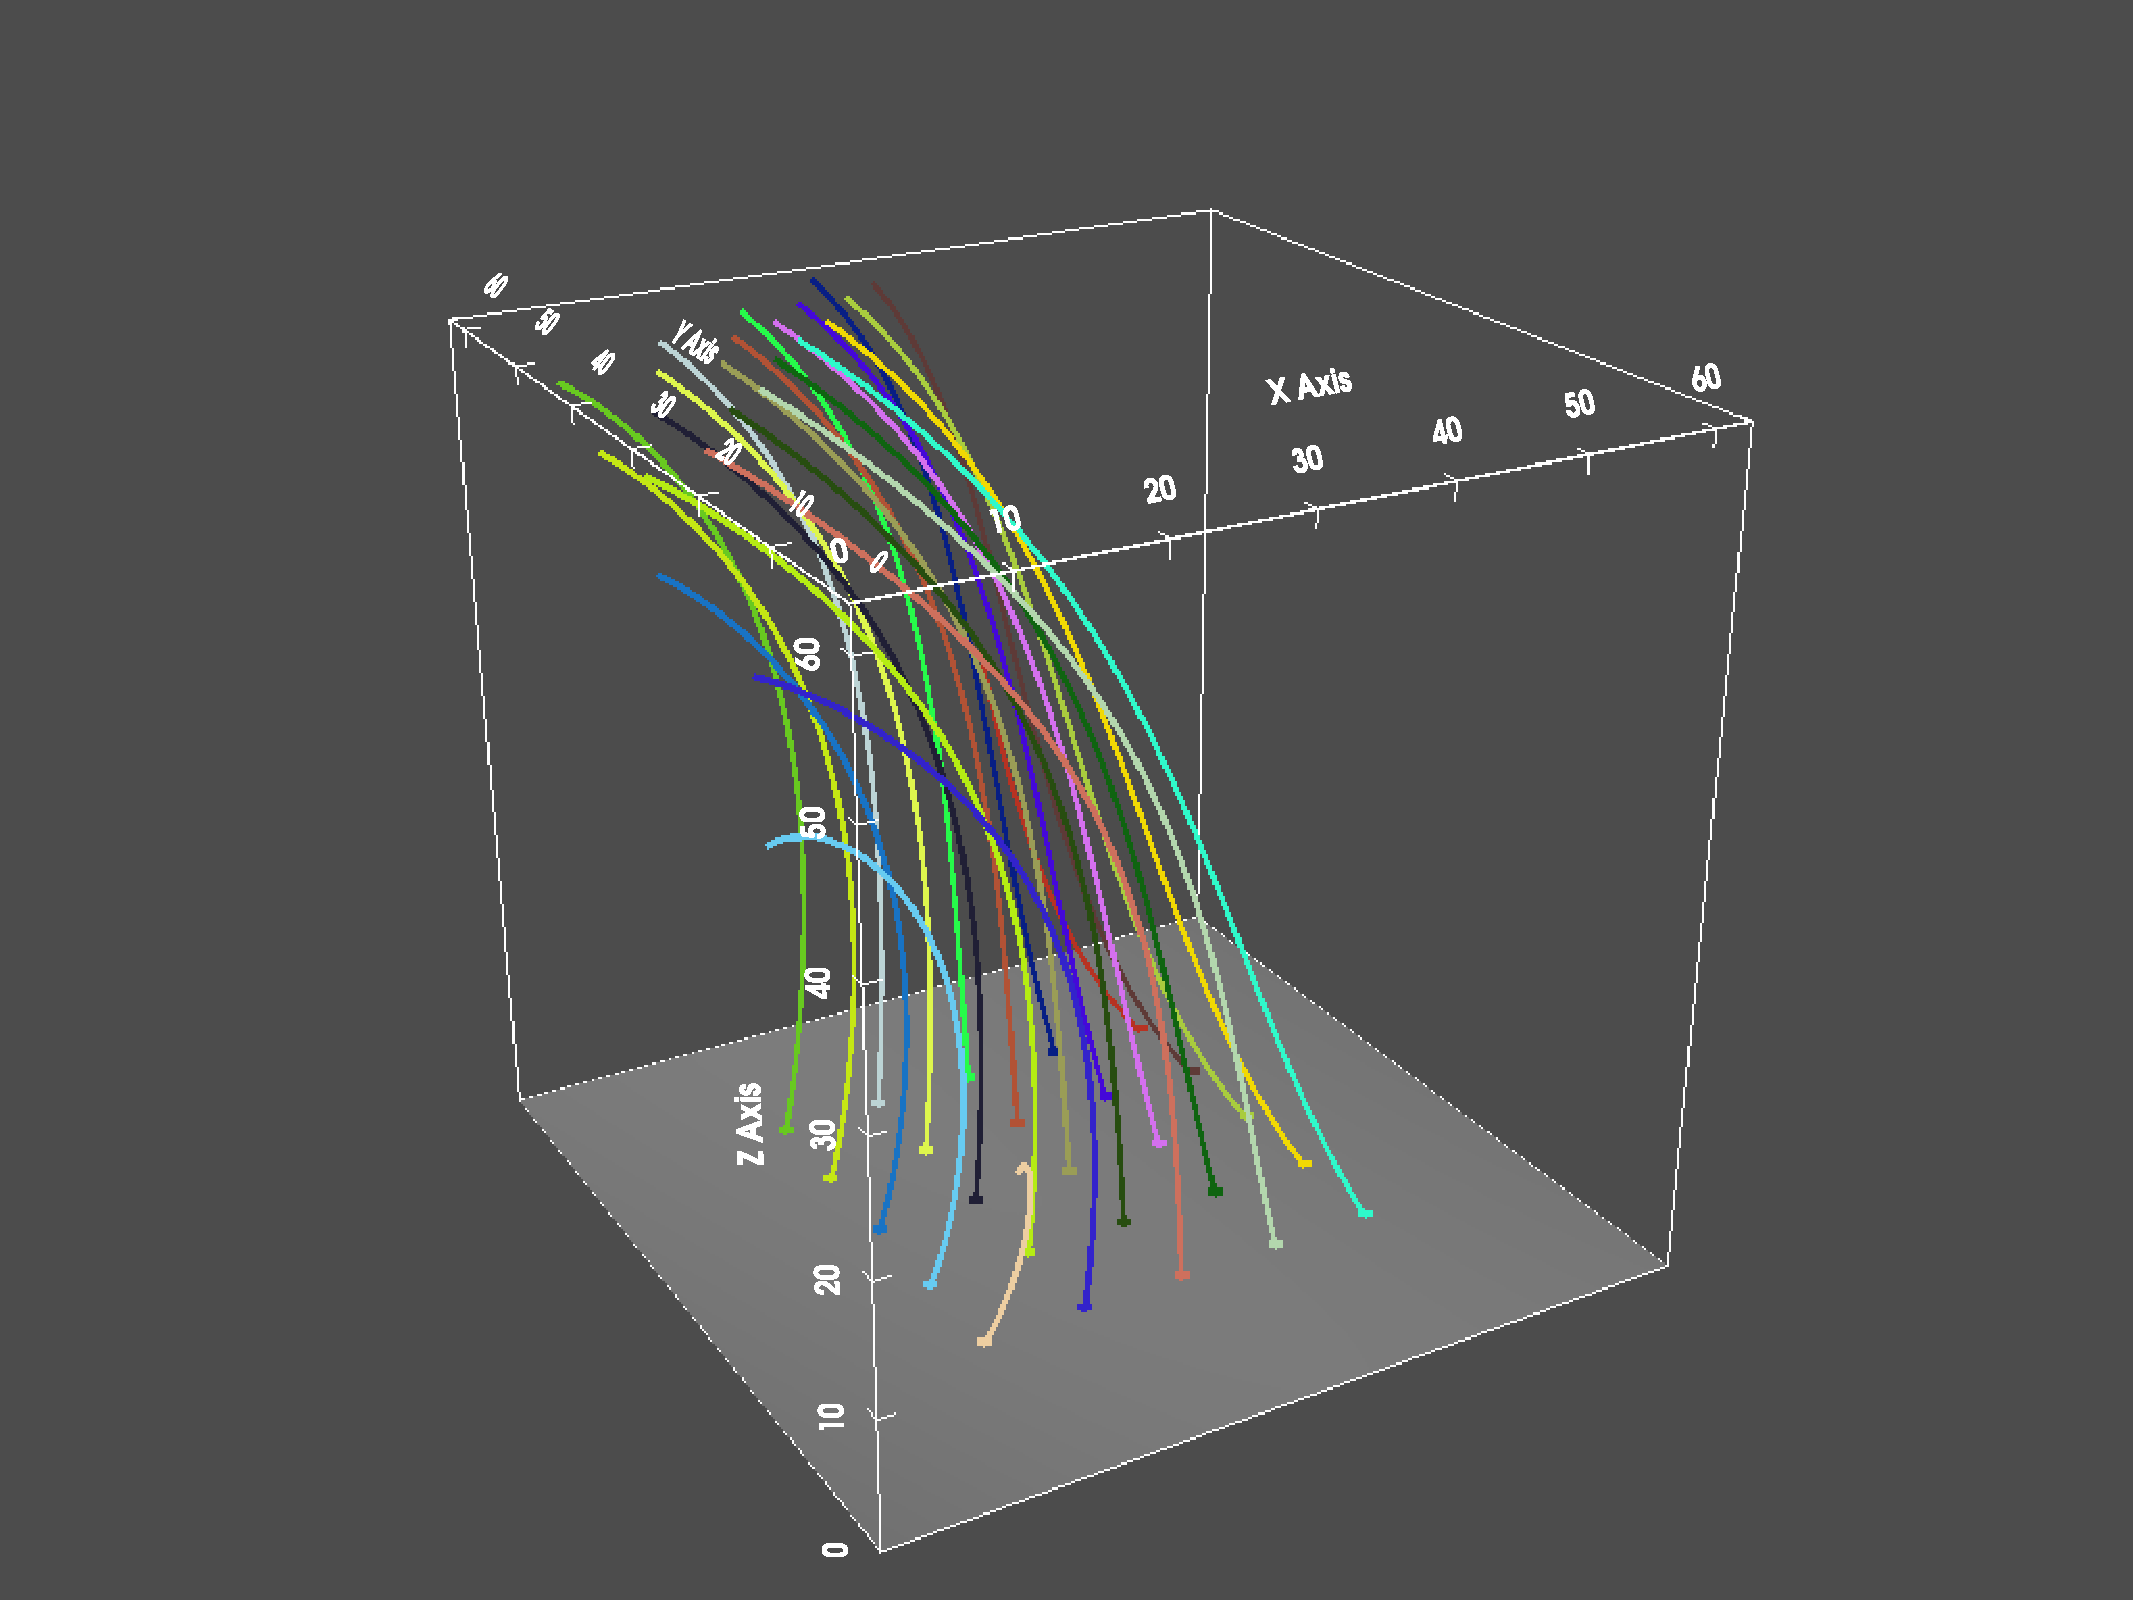
\includegraphics[trim={6cm 0cm 6cm 3cm}, clip, width=\linewidth]{"../../Thesis/img/PINN_000100_xz_tilted.pdf"}
            \end{subfigure}%
            \begin{subfigure}{.5\linewidth}
                \centering
                \caption{\large Low-Lou}
                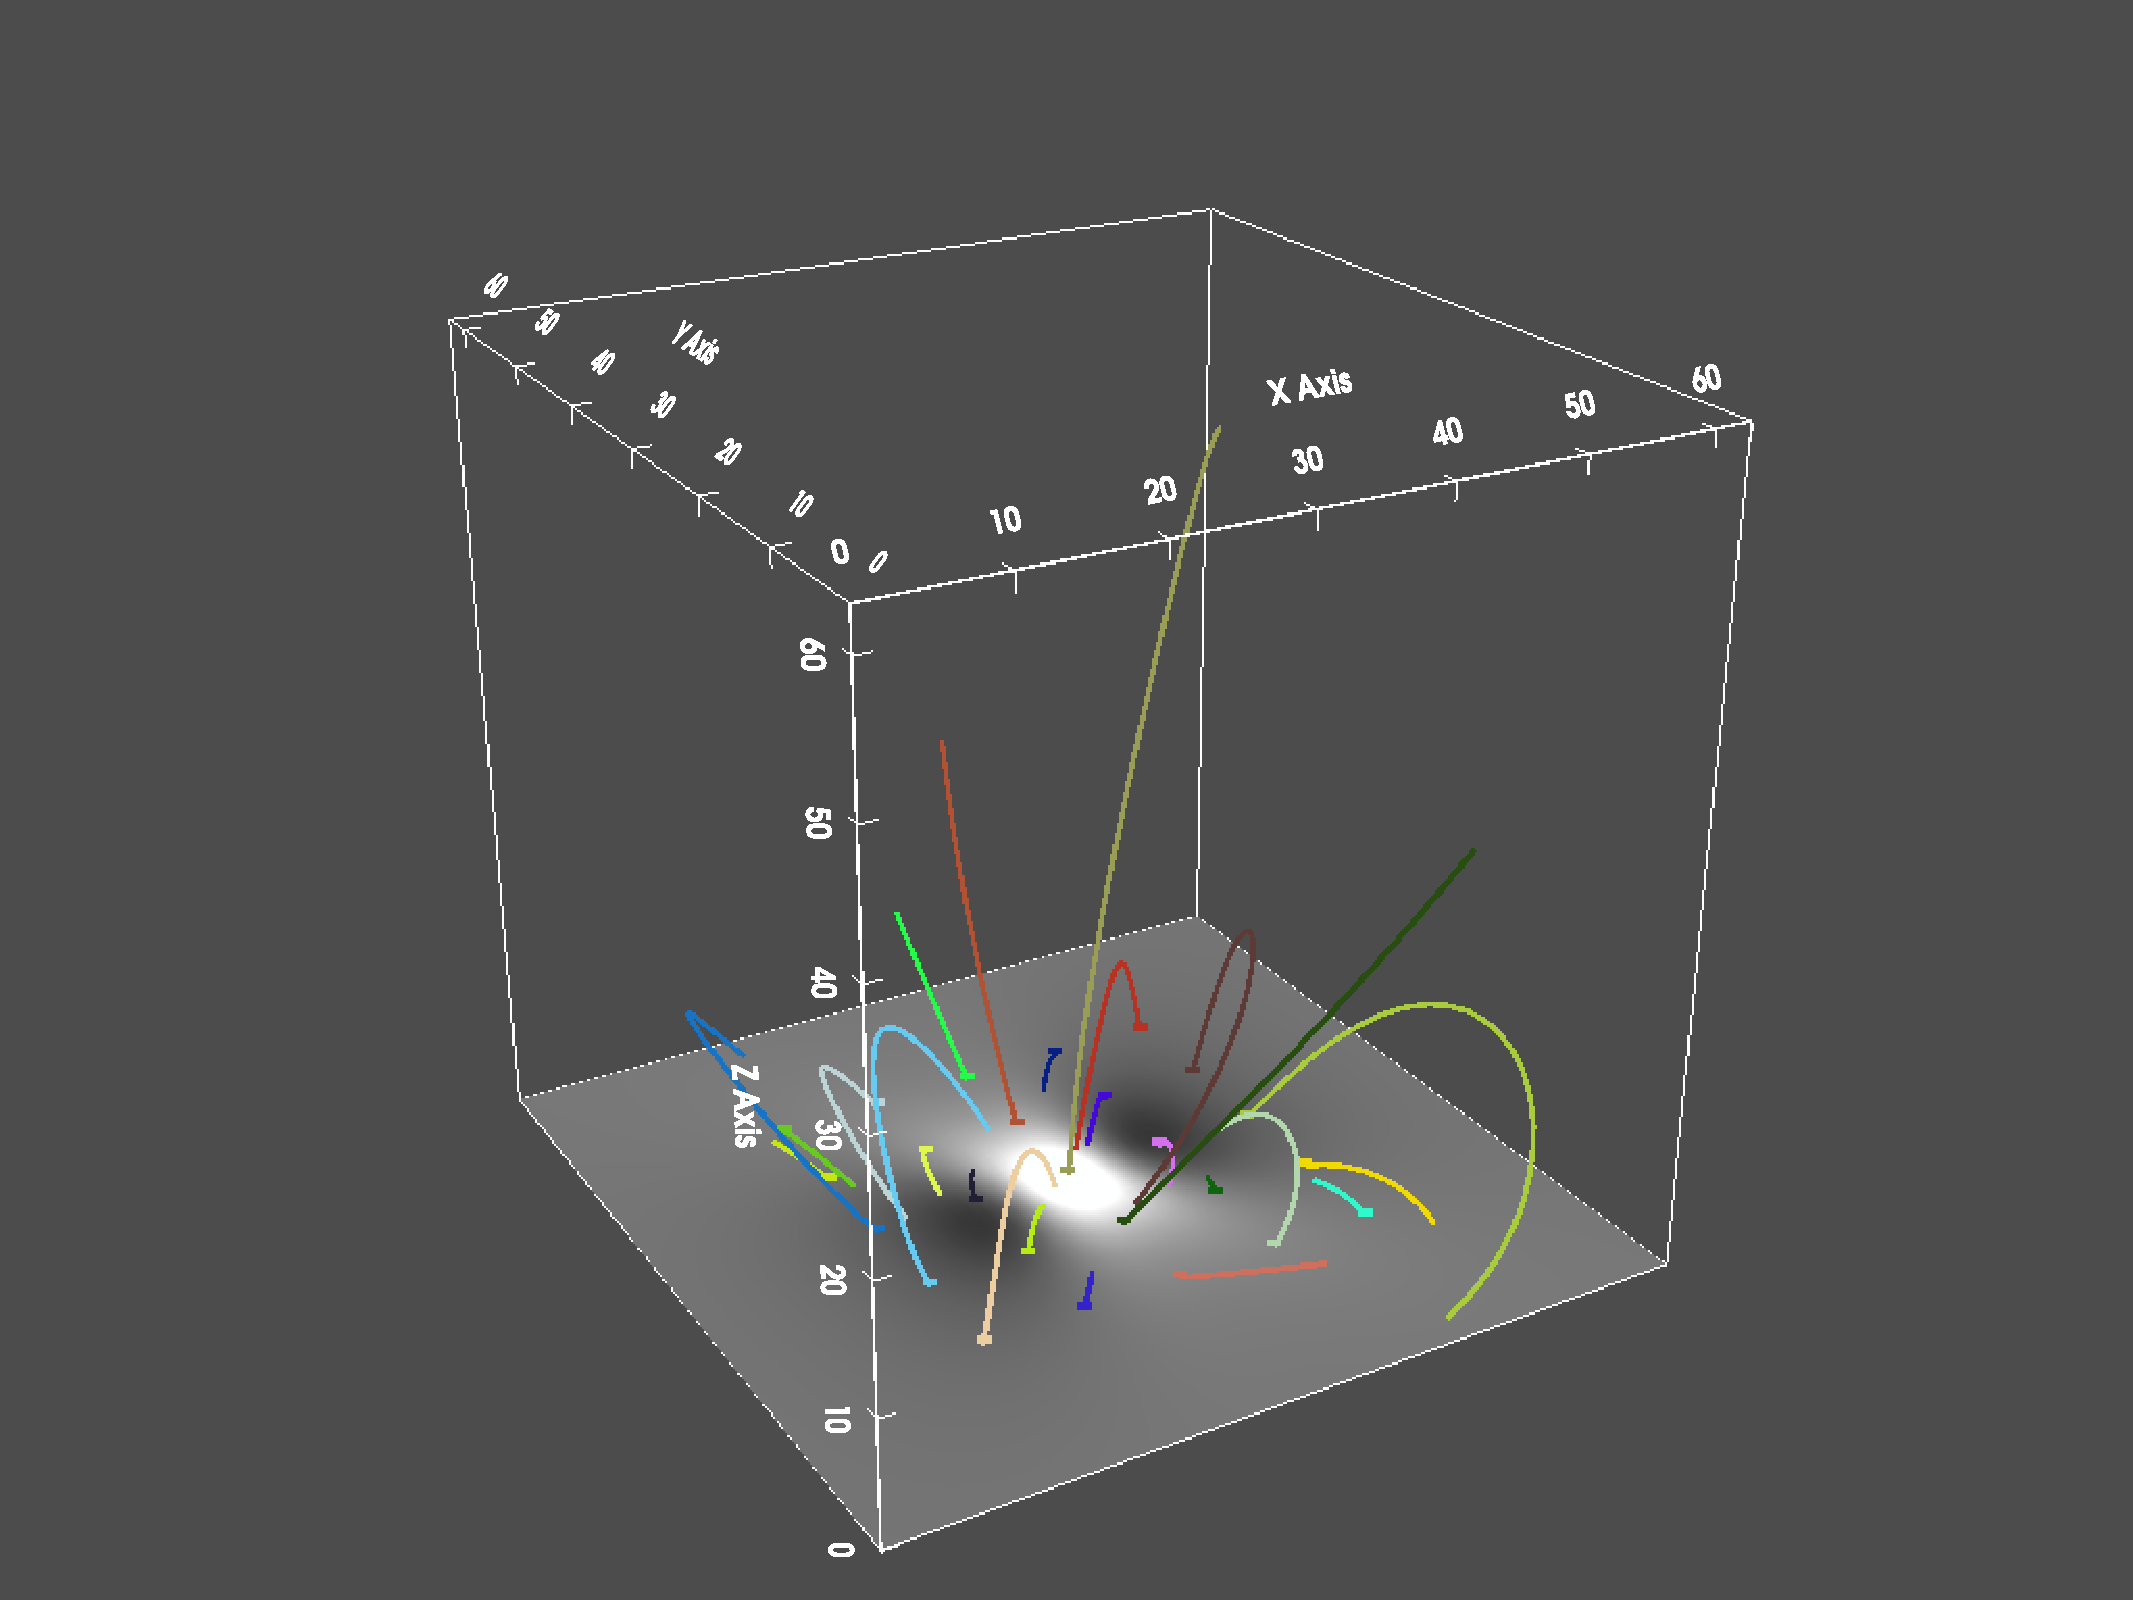
\includegraphics[trim={6cm 0cm 6cm 3cm}, clip, width=\linewidth]{"../../Thesis/img/LL_xz_tilted.pdf"}
              \end{subfigure}
            }
            
            \only<3>{
                \begin{subfigure}{.5\linewidth}
              \centering
              \caption{\large PINN(1000)}
              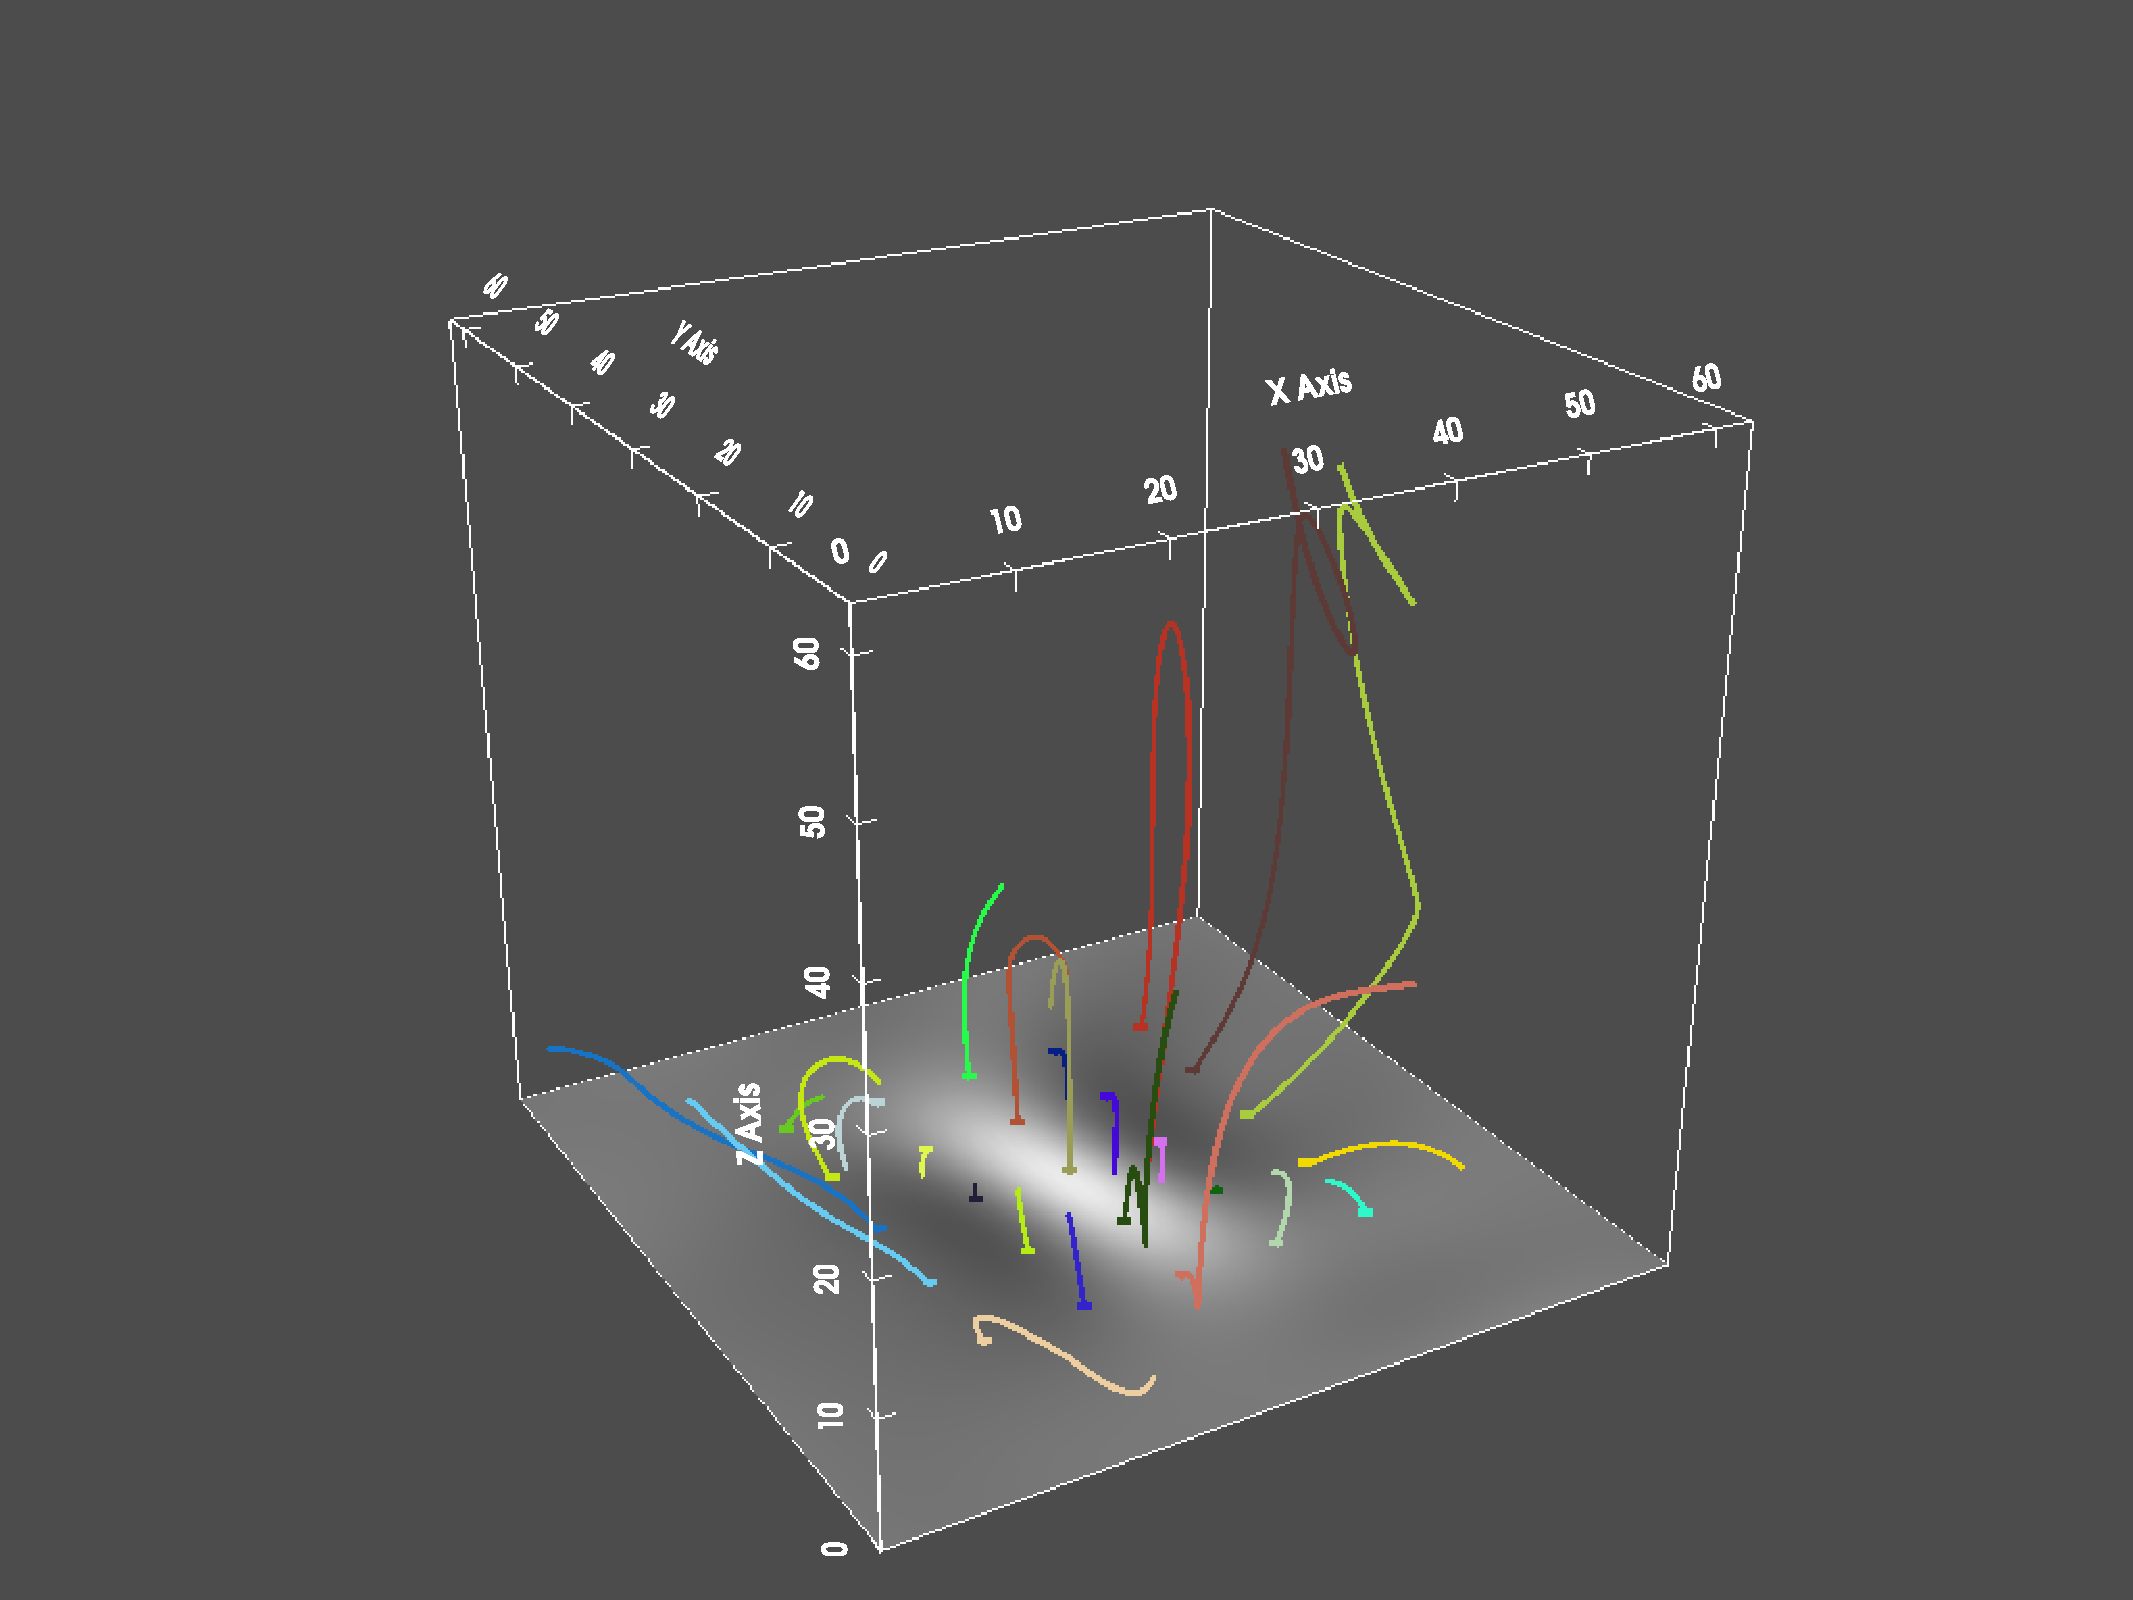
\includegraphics[trim={6cm 0cm 6cm 3cm}, clip, width=\linewidth]{"../../Thesis/img/PINN_001000_xz_tilted.pdf"}
            \end{subfigure}%
            \begin{subfigure}{.5\linewidth}
                \centering
                \caption{\large Low-Lou}
                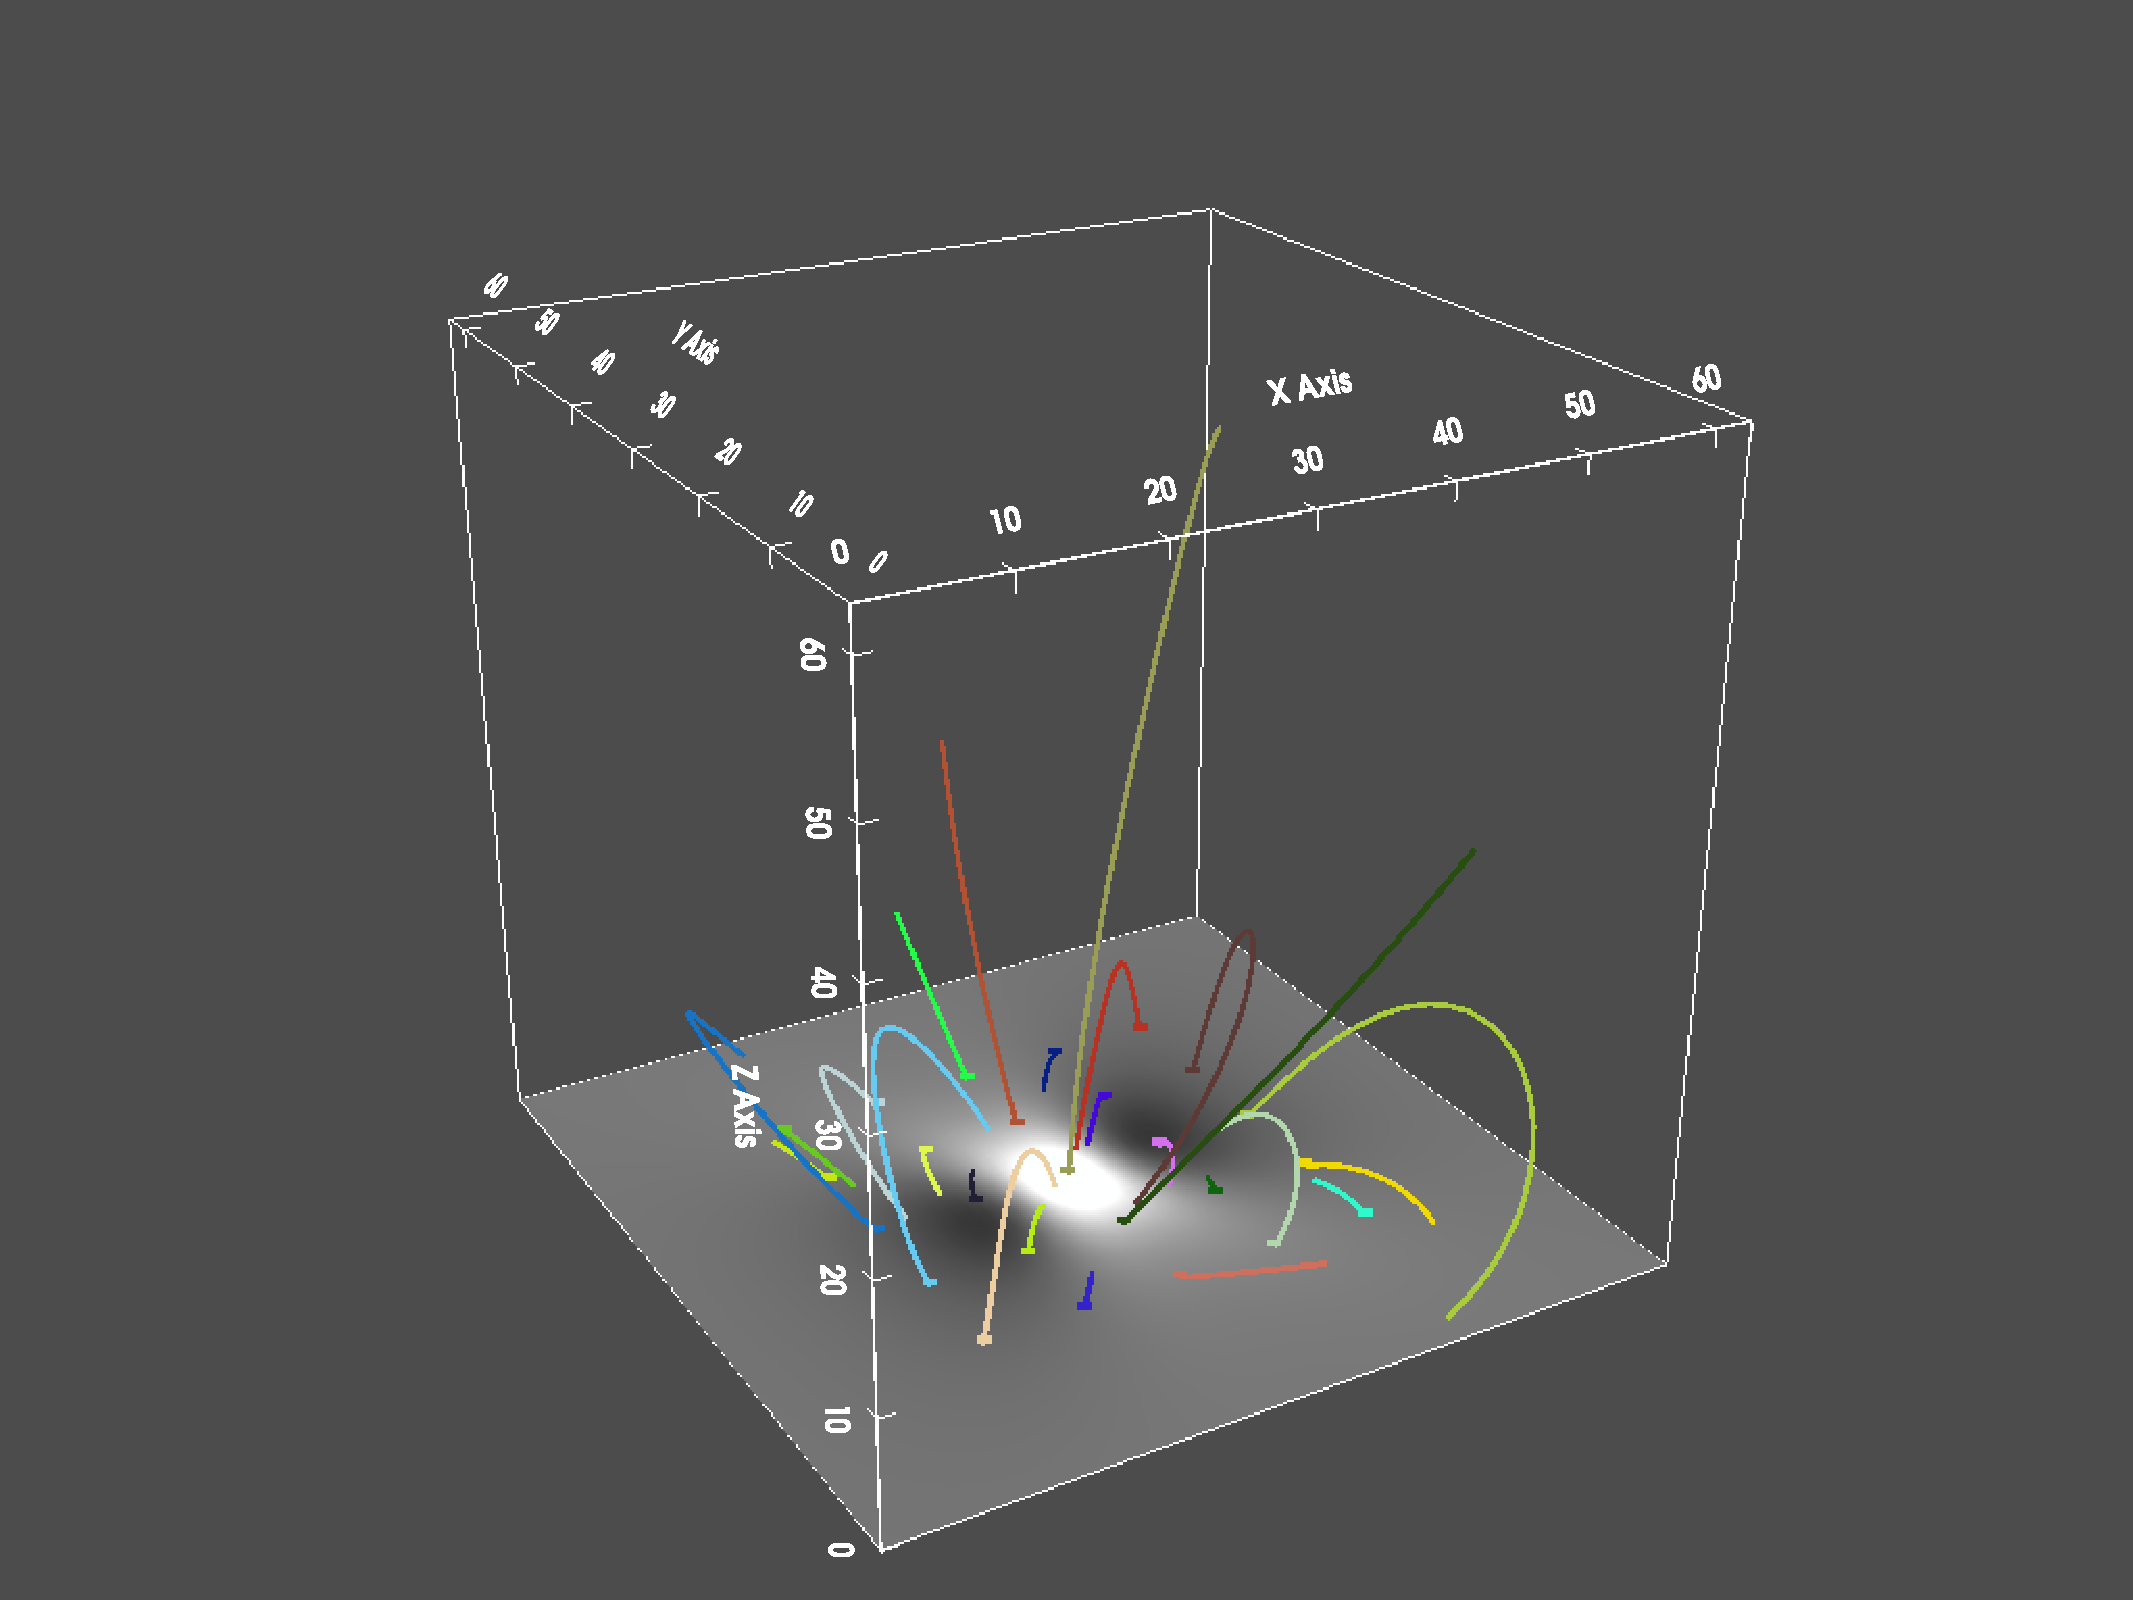
\includegraphics[trim={6cm 0cm 6cm 3cm}, clip, width=\linewidth]{"../../Thesis/img/LL_xz_tilted.pdf"}
              \end{subfigure}
            }

            \only<4>{
            \begin{subfigure}{.5\linewidth}
              \centering
              \caption{\large PINN(10000)}
              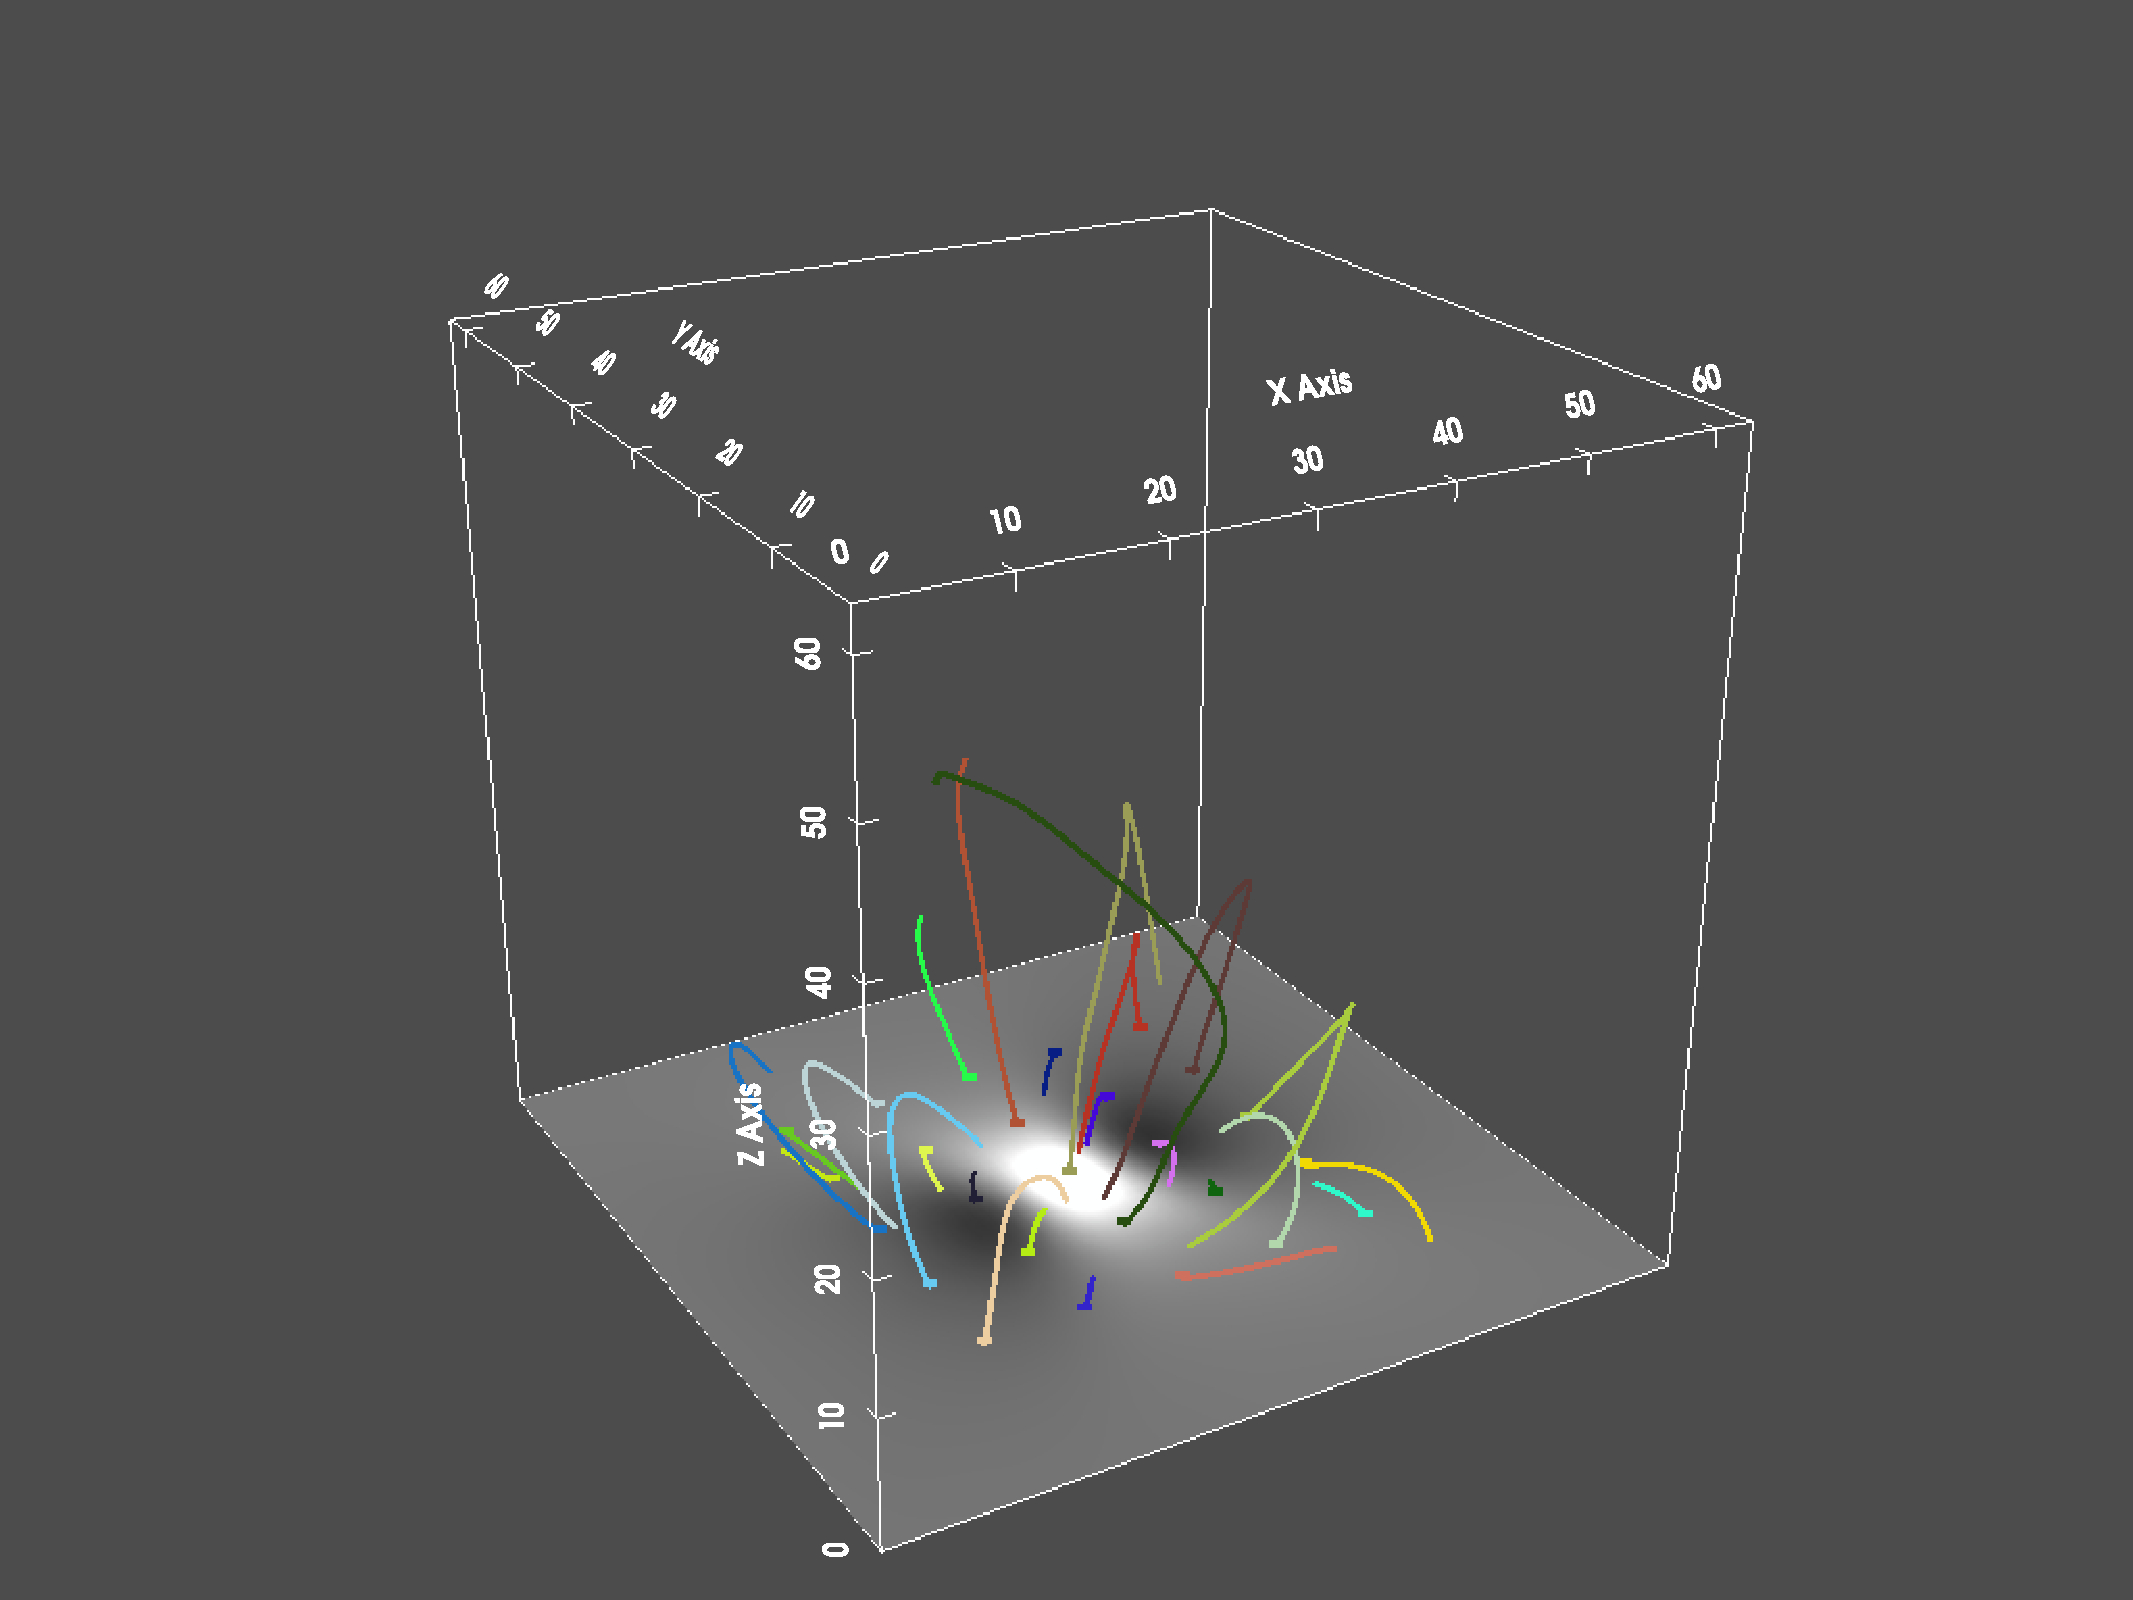
\includegraphics[trim={6cm 0cm 6cm 3cm}, clip, width=\linewidth]{"../../Thesis/img/PINN_010000_xz_tilted.pdf"}
            \end{subfigure}%
            \begin{subfigure}{.5\linewidth}
                \centering
                \caption{\large Low-Lou}
                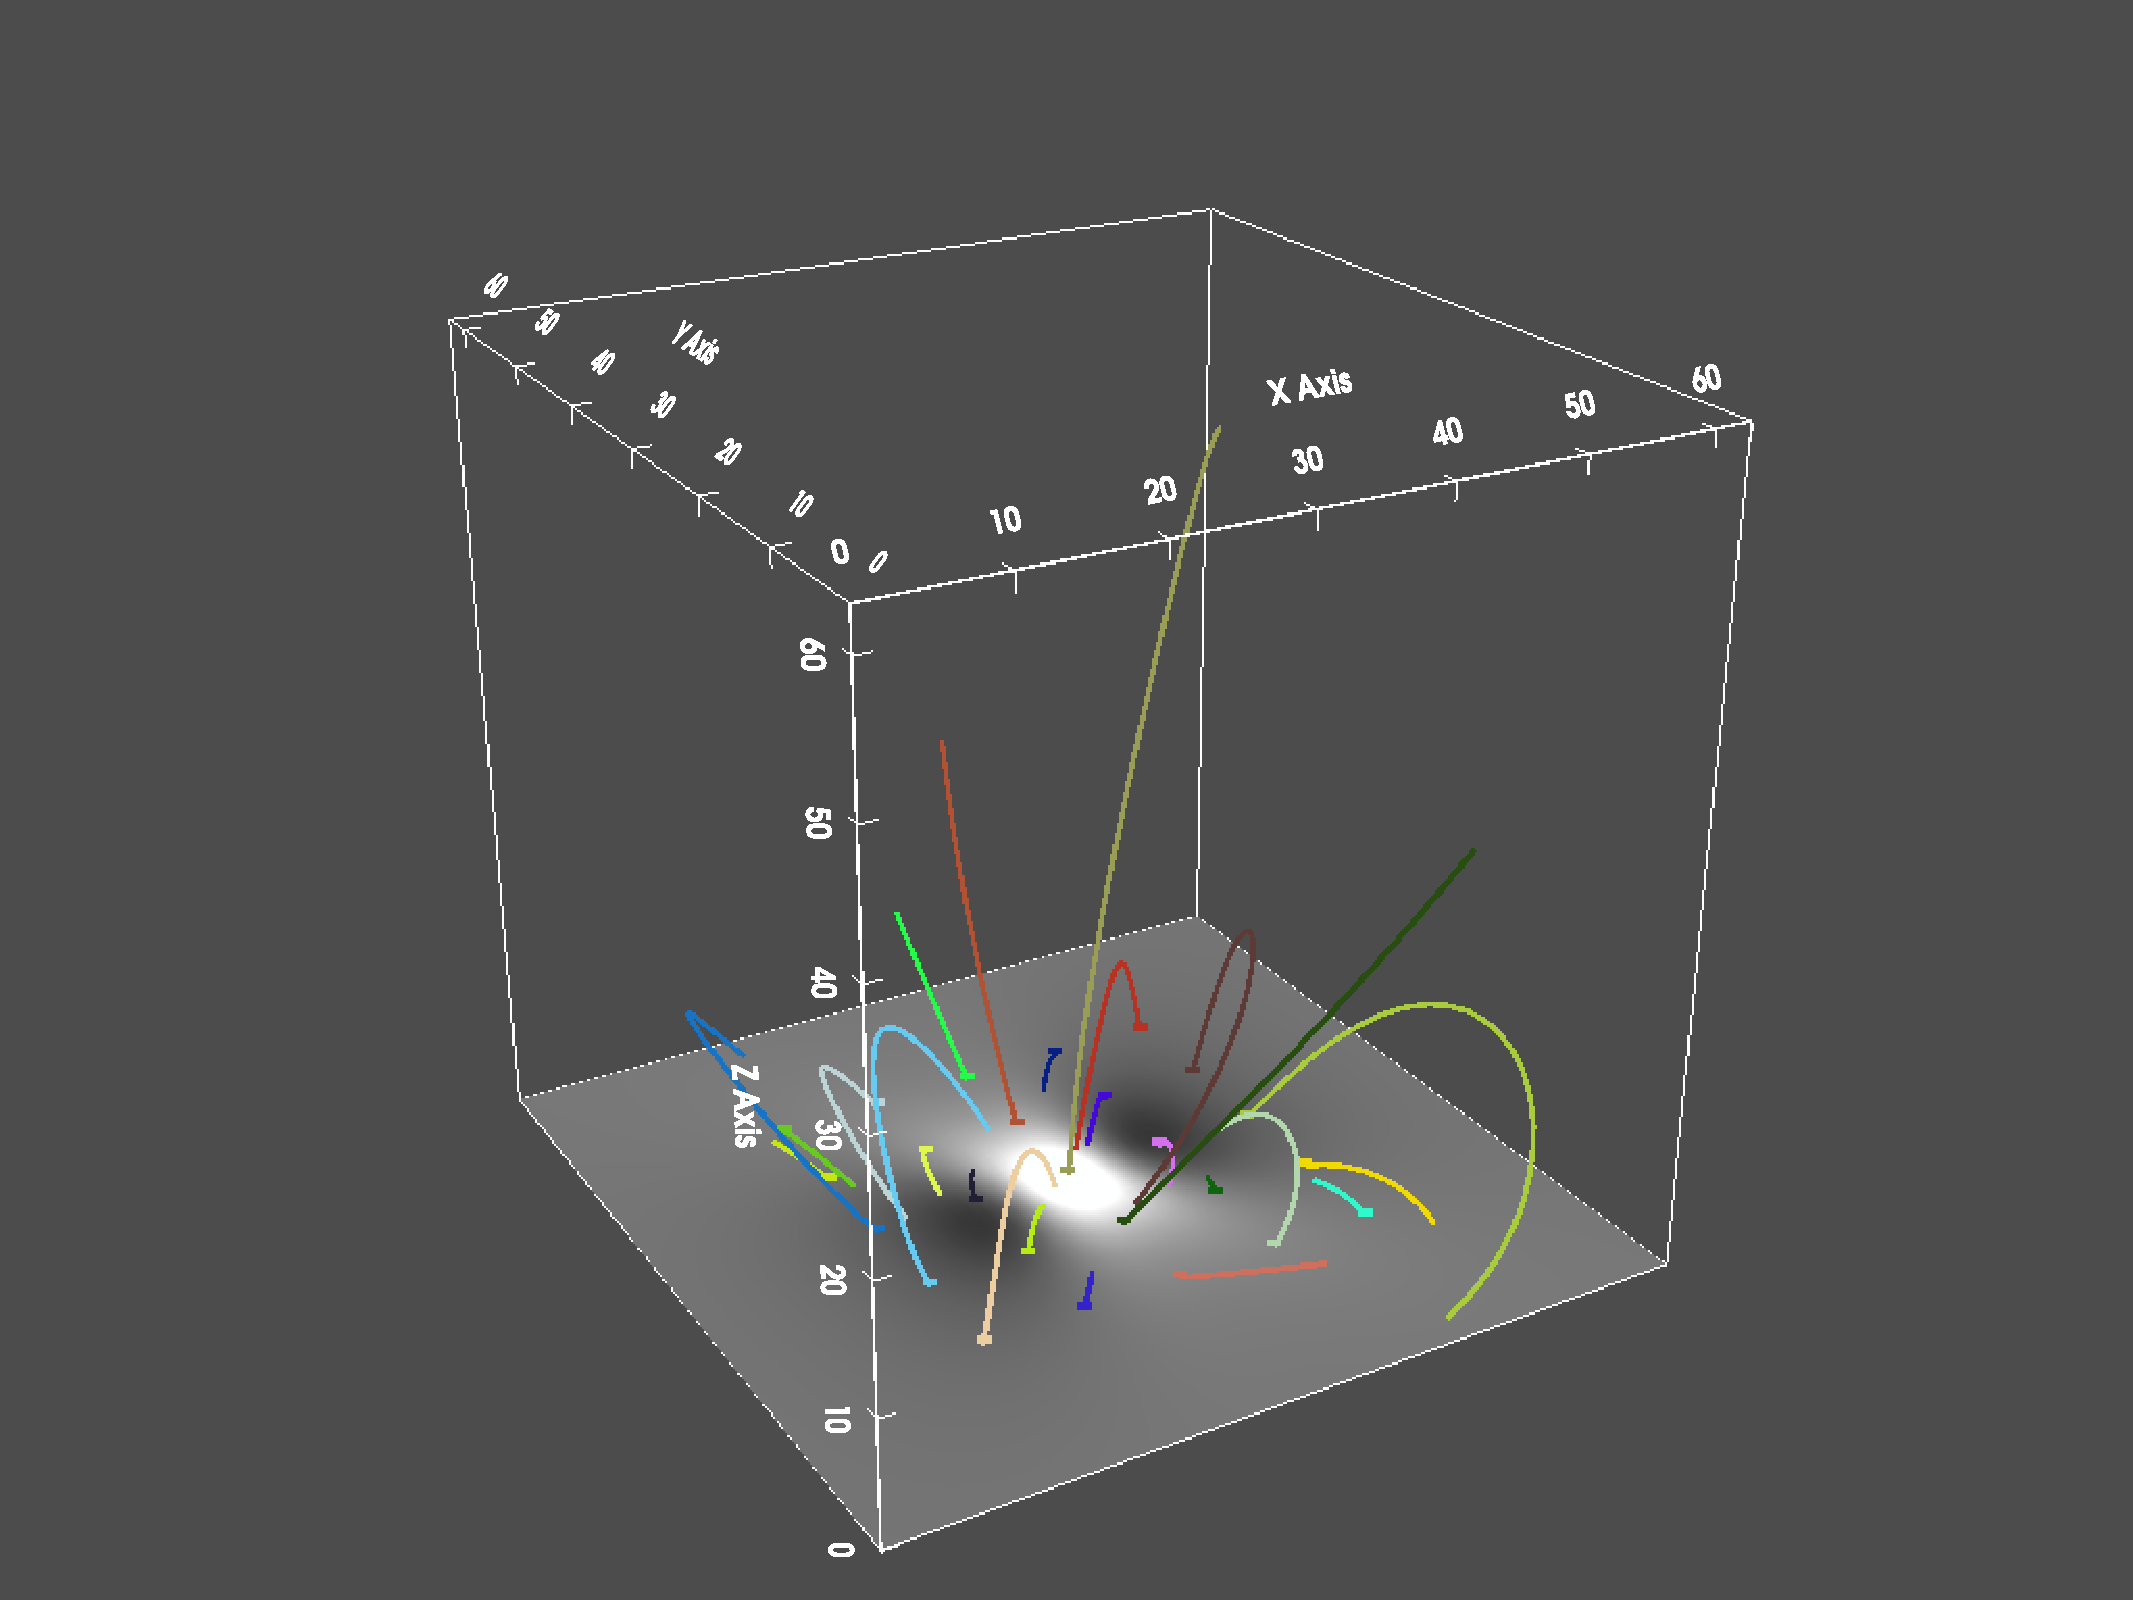
\includegraphics[trim={6cm 0cm 6cm 3cm}, clip, width=\linewidth]{"../../Thesis/img/LL_xz_tilted.pdf"}
              \end{subfigure}
            }
    
            \only<5>{\begin{subfigure}{.5\linewidth}
                \centering
                \caption{\large PINN(25000)}
                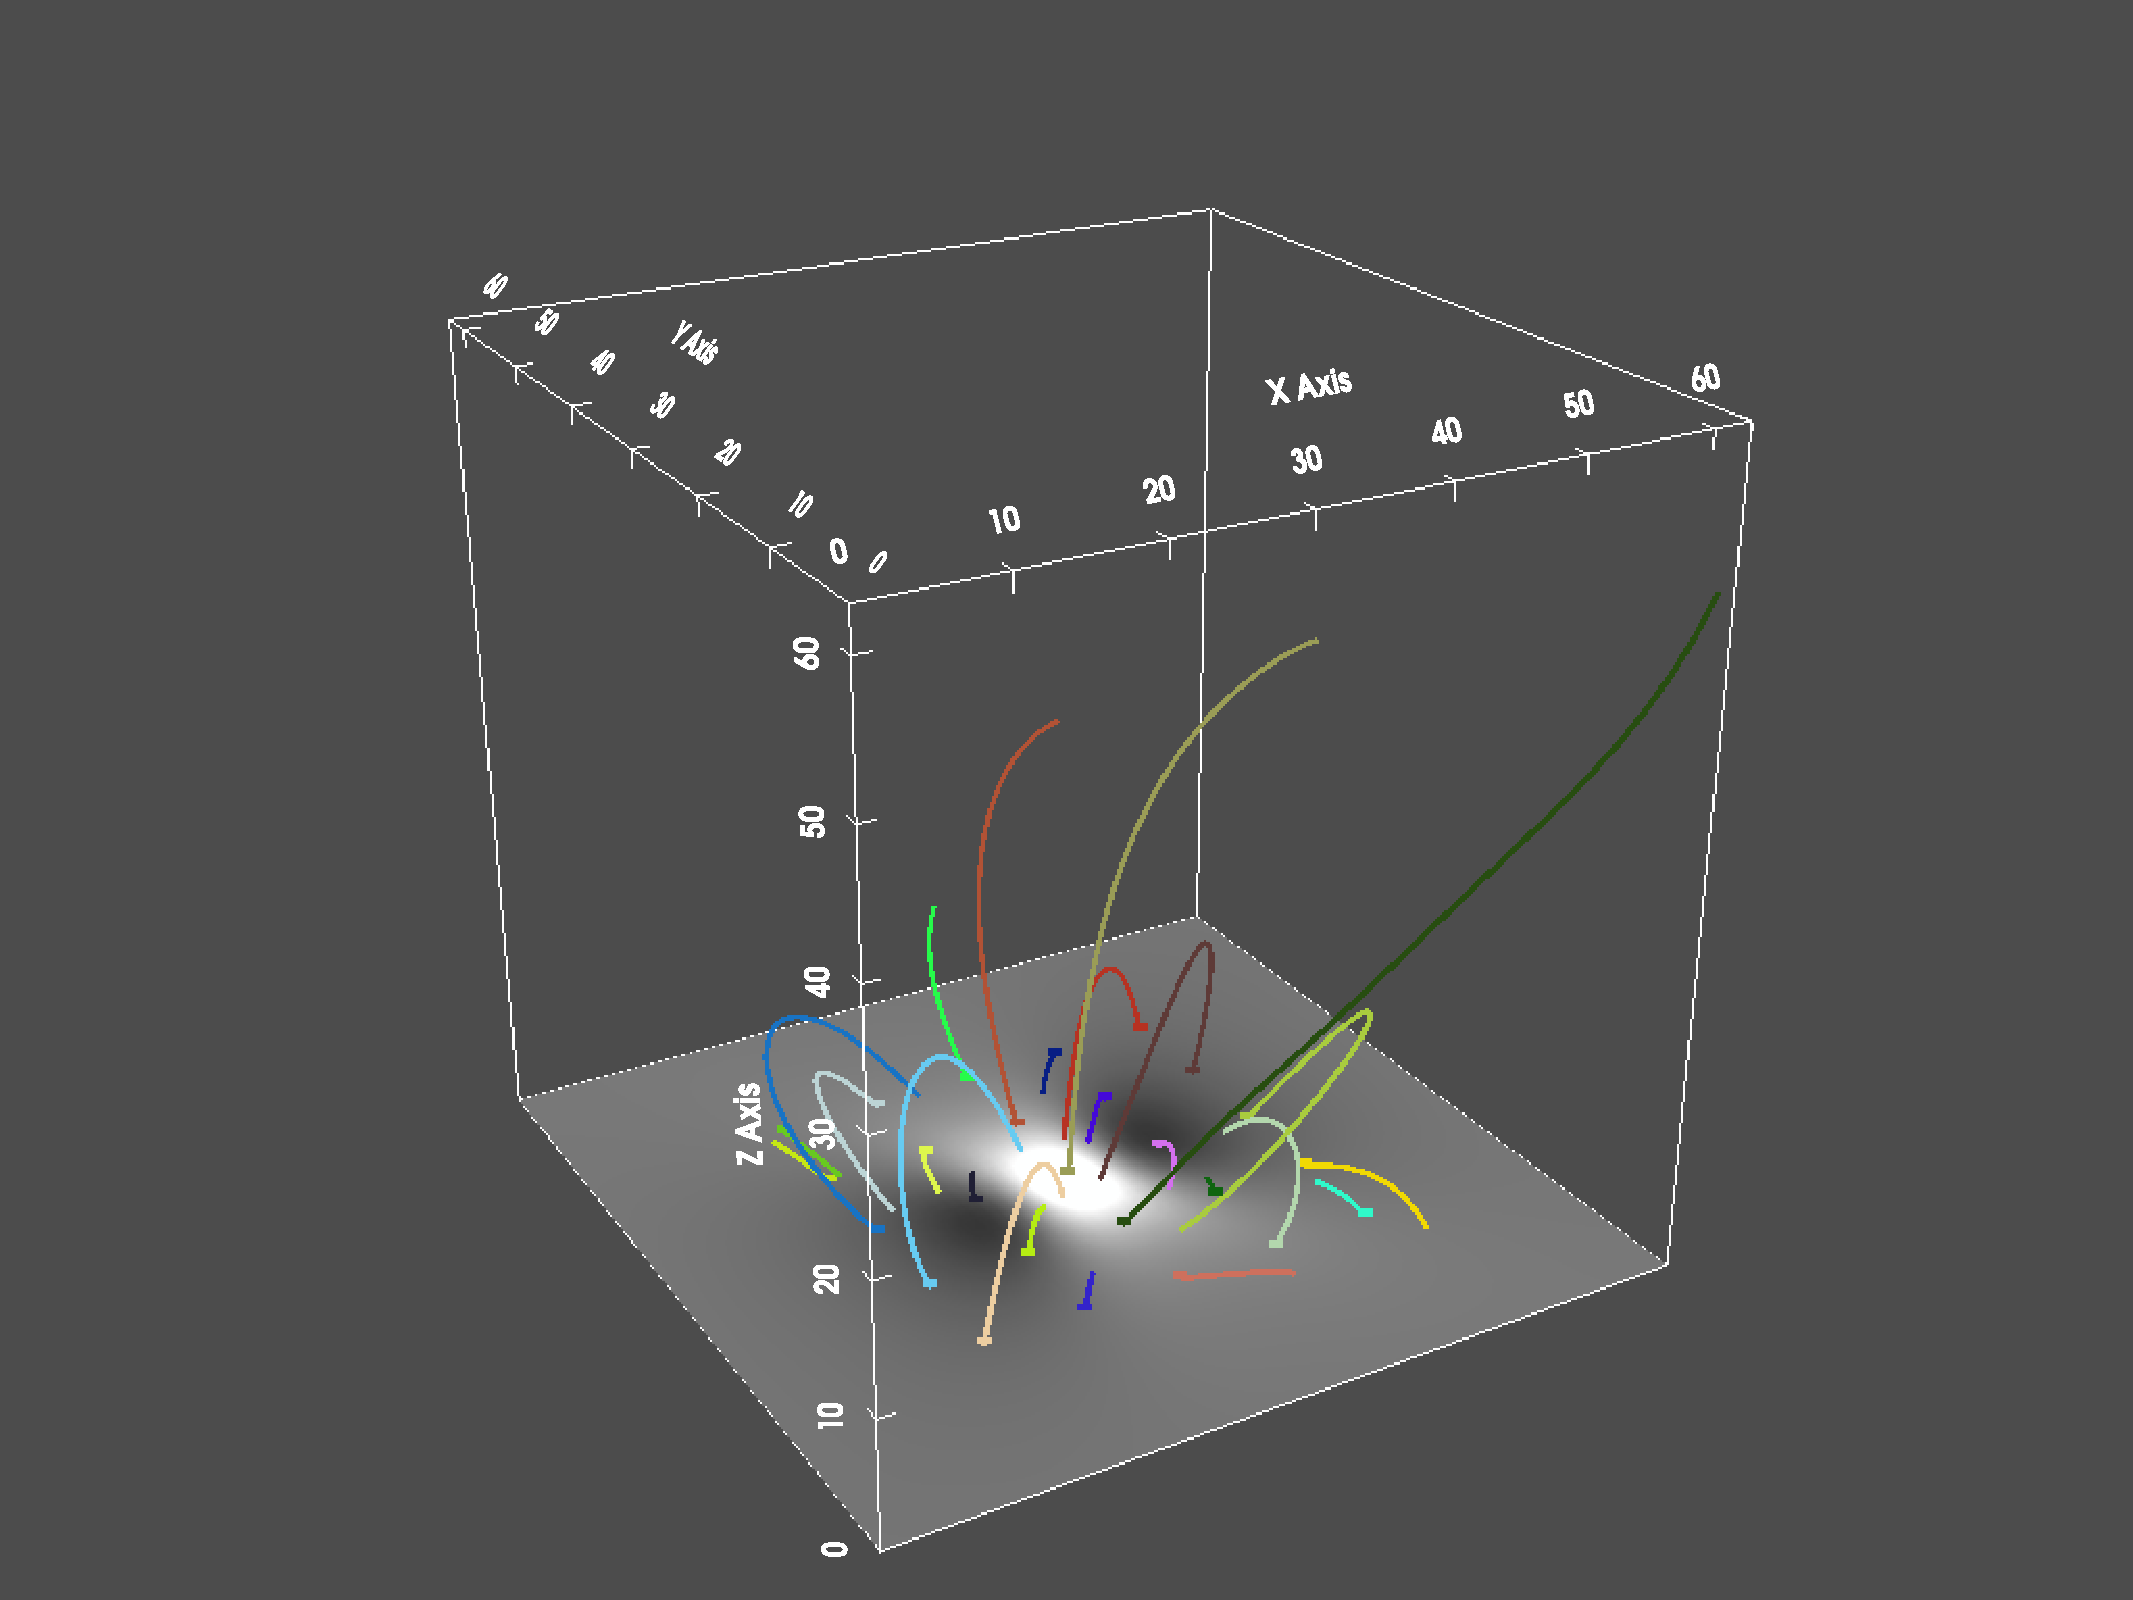
\includegraphics[trim={6cm 0cm 6cm 3cm}, clip, width=\linewidth]{"../../Thesis/img/PINN_025000_xz_tilted.pdf"}
              \end{subfigure}%
              \begin{subfigure}{.5\linewidth}
                \centering
                \caption{\large Low-Lou}
                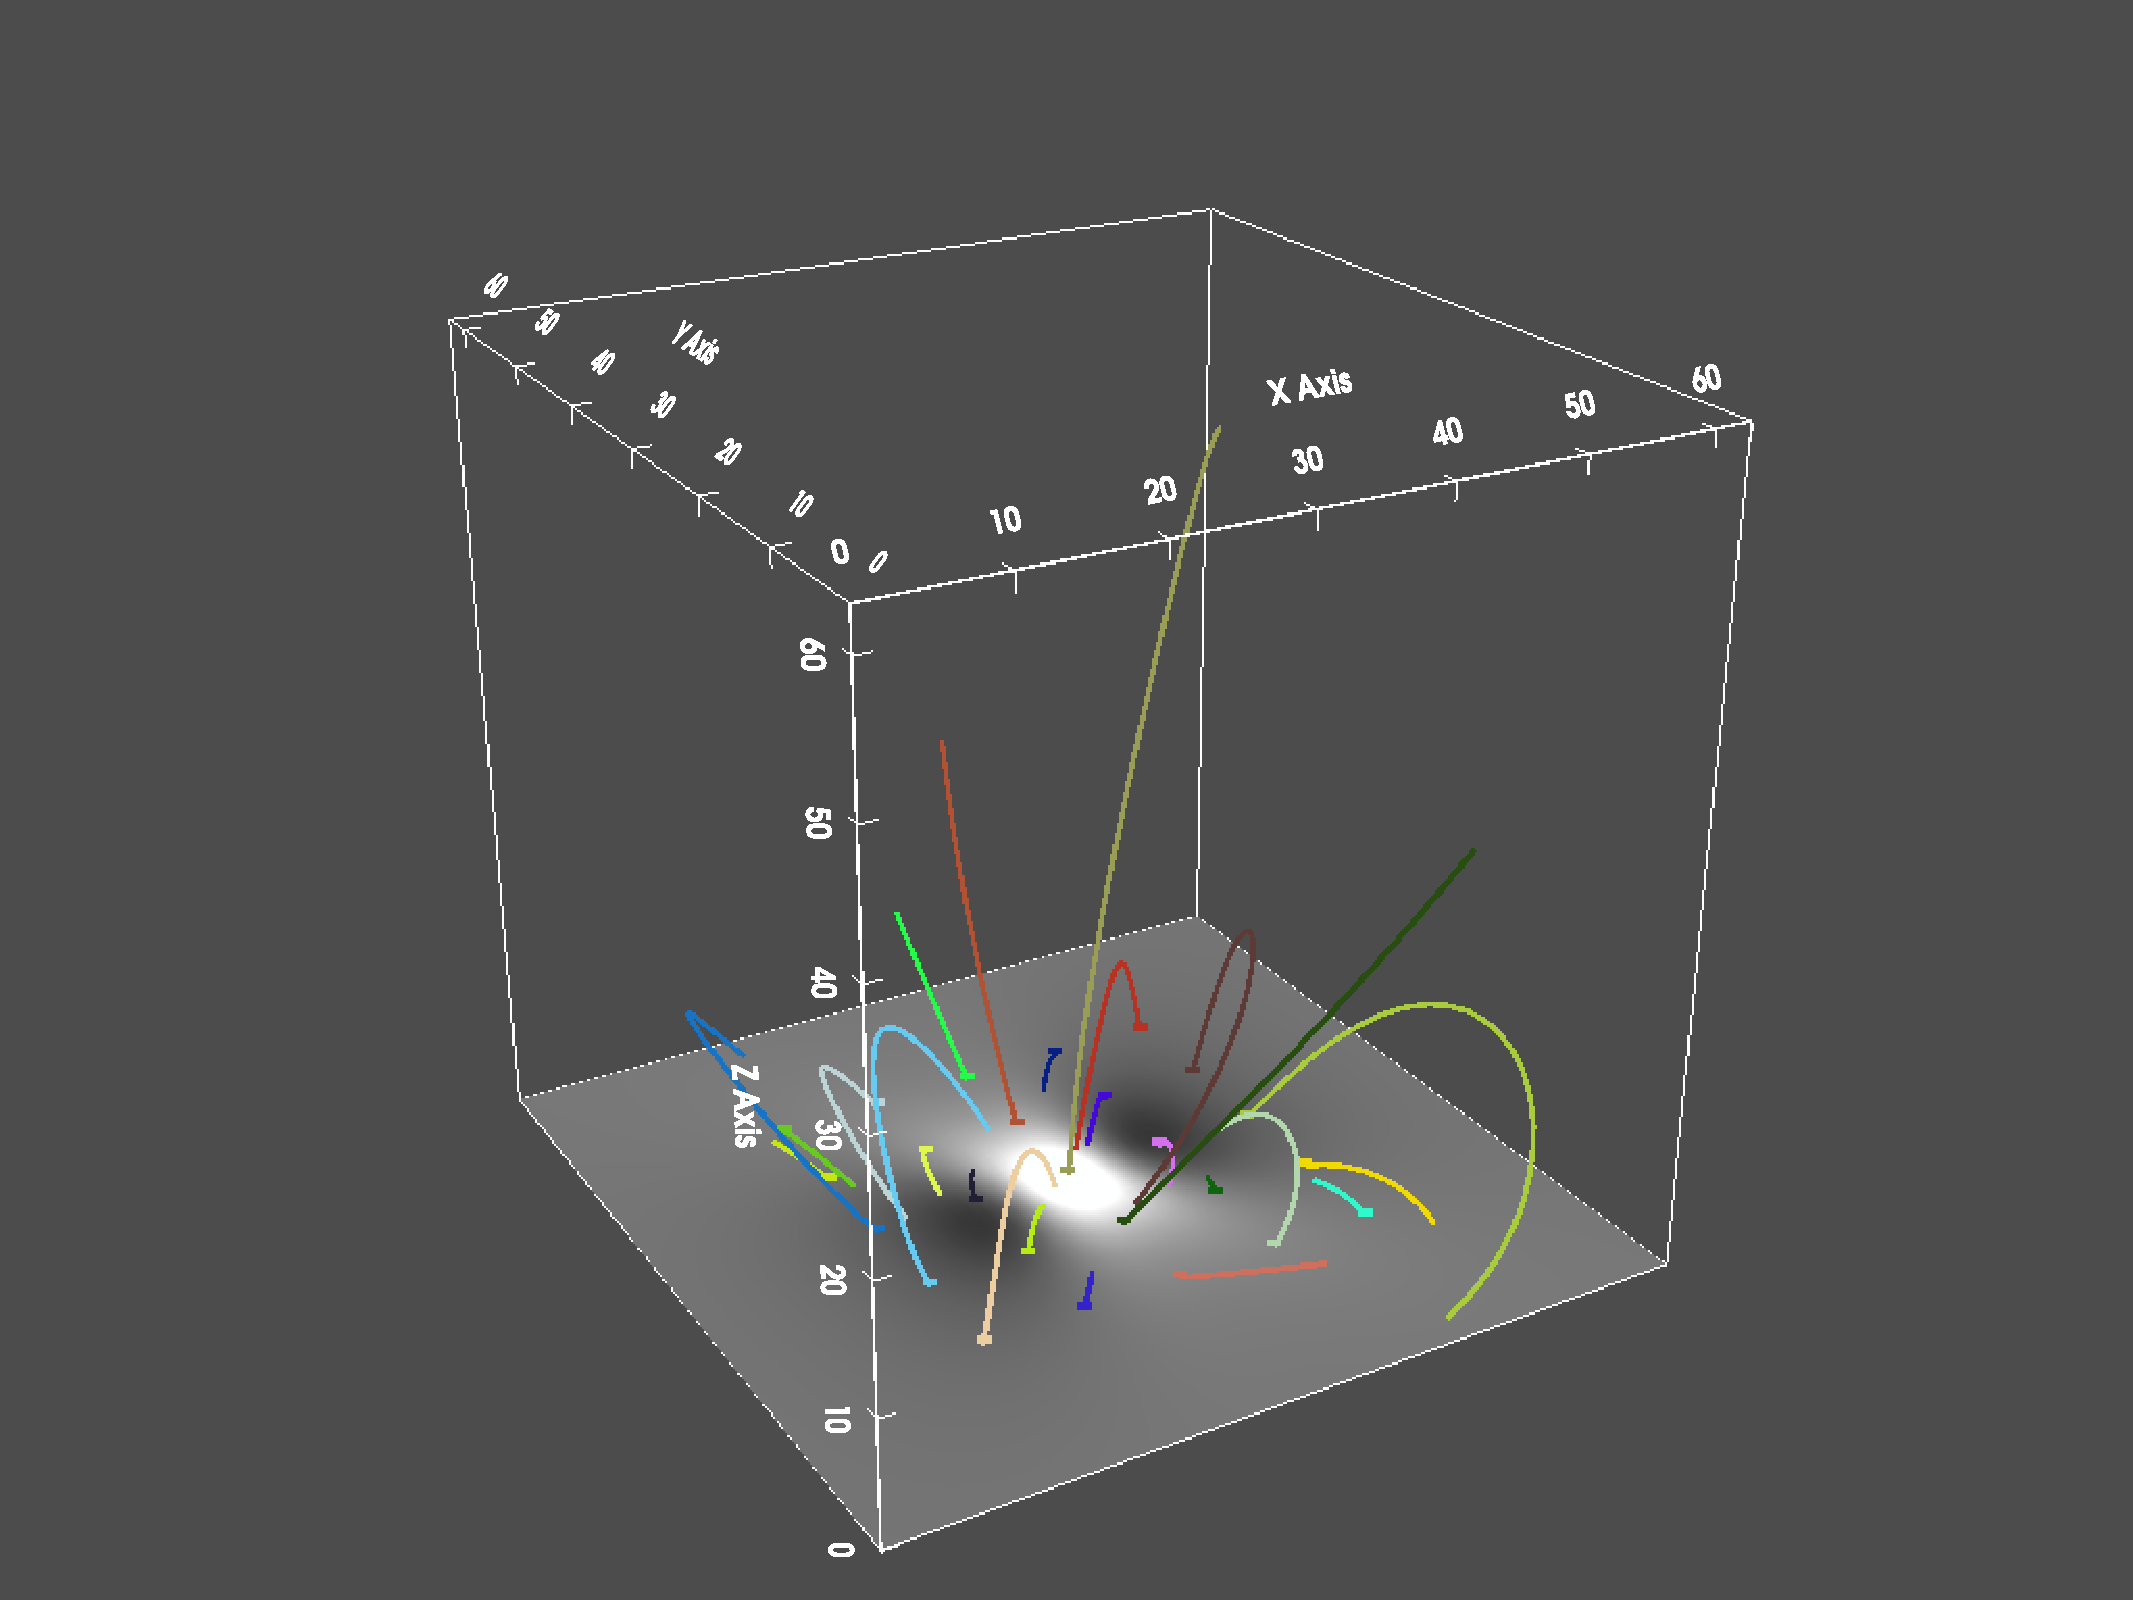
\includegraphics[trim={6cm 0cm 6cm 3cm}, clip, width=\linewidth]{"../../Thesis/img/LL_xz_tilted.pdf"}
              \end{subfigure}
              }

            \only<6>{\begin{subfigure}{.5\linewidth}
                \centering
                \caption{\large PINN(50000)}
                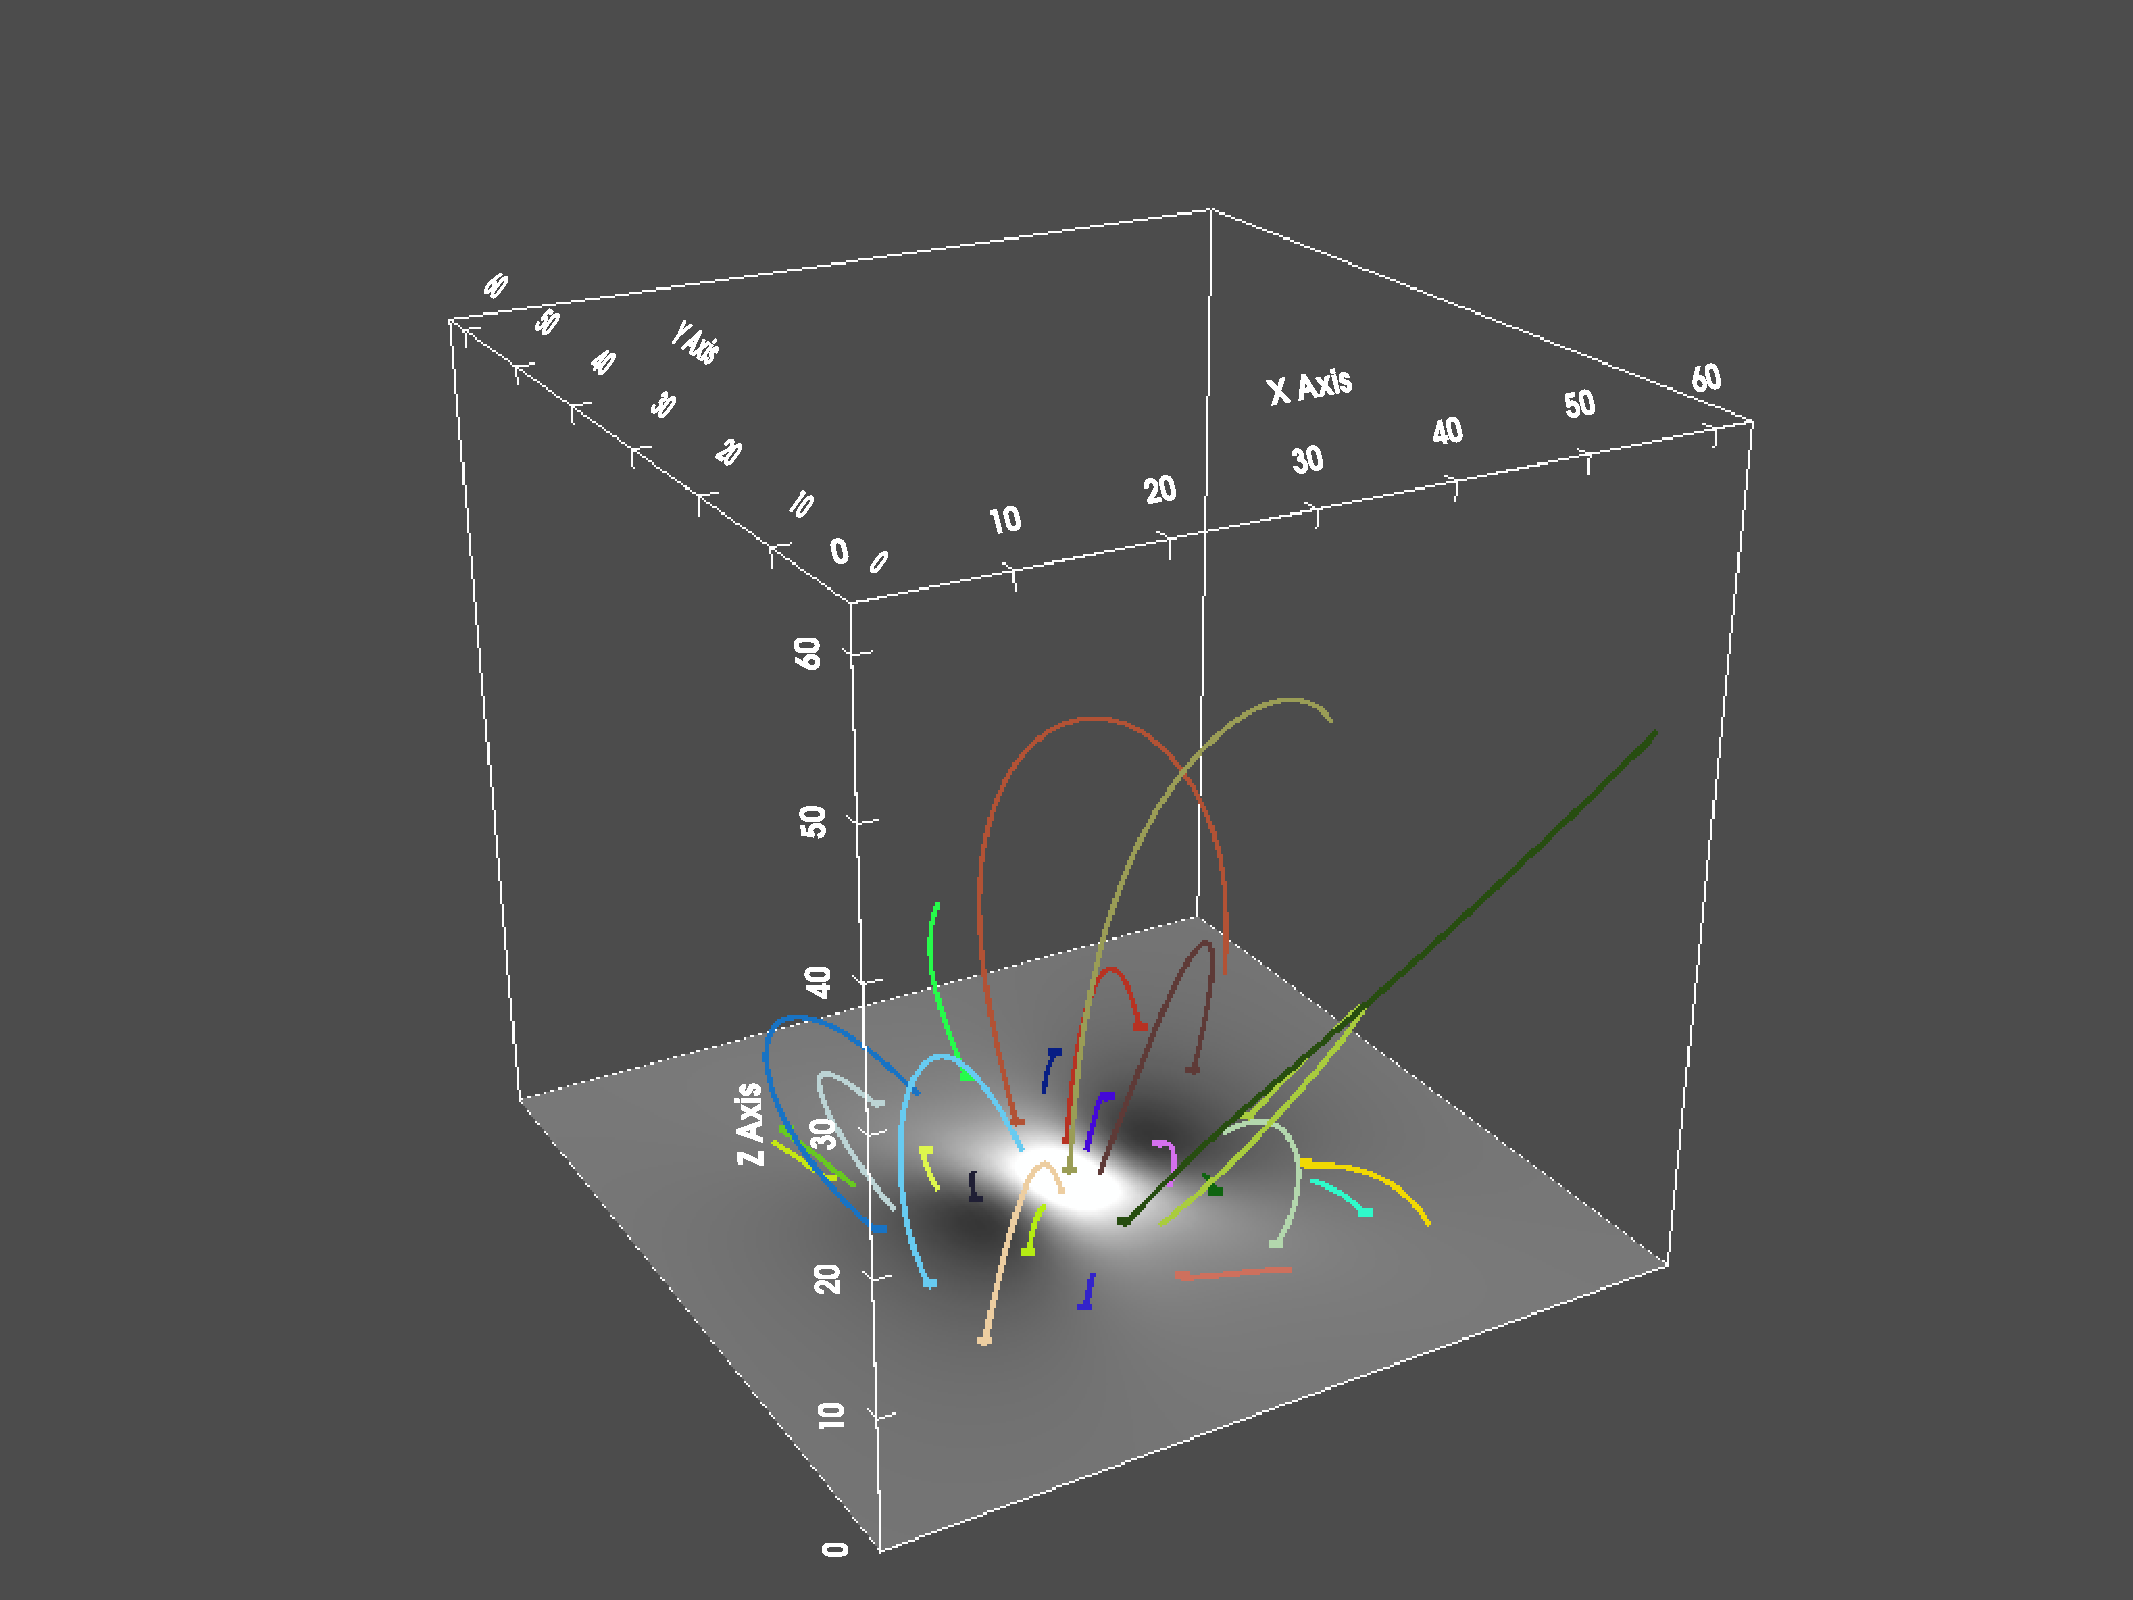
\includegraphics[trim={6cm 0cm 6cm 3cm}, clip, width=\linewidth]{"../../Thesis/img/PINN_050000_xz_tilted.pdf"}
              \end{subfigure}%
              \begin{subfigure}{.5\linewidth}
                \centering
                \caption{\large Low-Lou}
                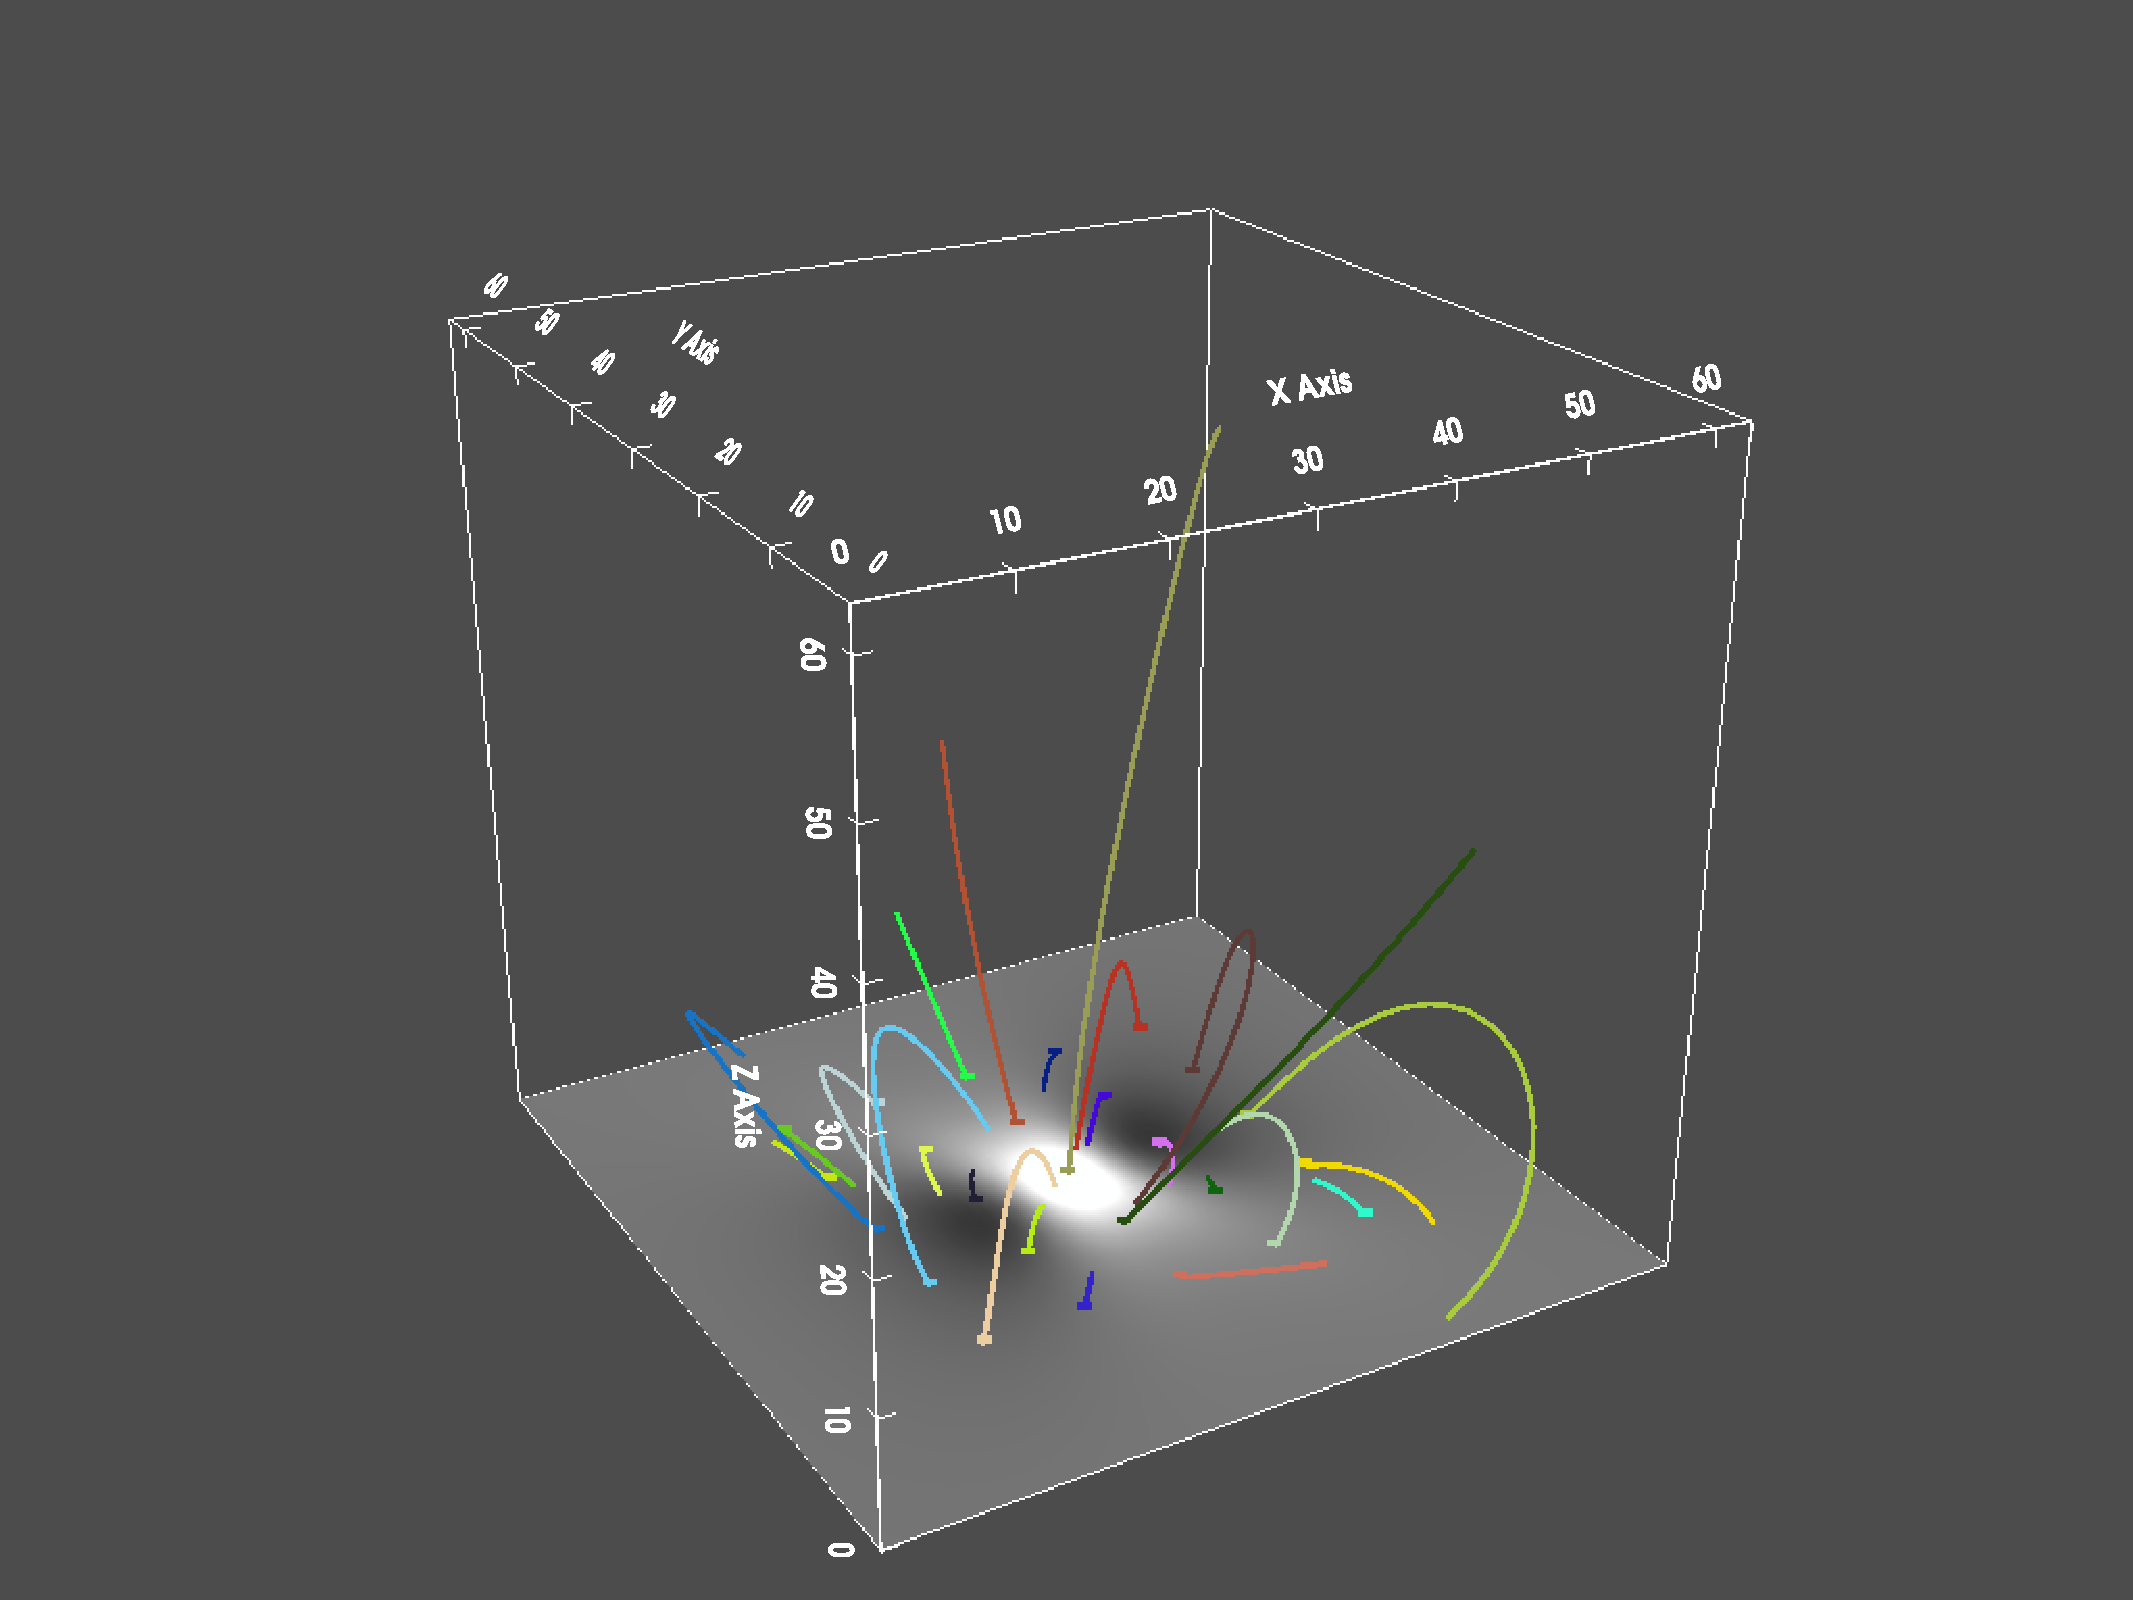
\includegraphics[trim={6cm 0cm 6cm 3cm}, clip, width=\linewidth]{"../../Thesis/img/LL_xz_tilted.pdf"}
              \end{subfigure}
              }
            
            \only<7>{\begin{subfigure}{.5\linewidth}
              \centering
              \caption{\large Potential}
              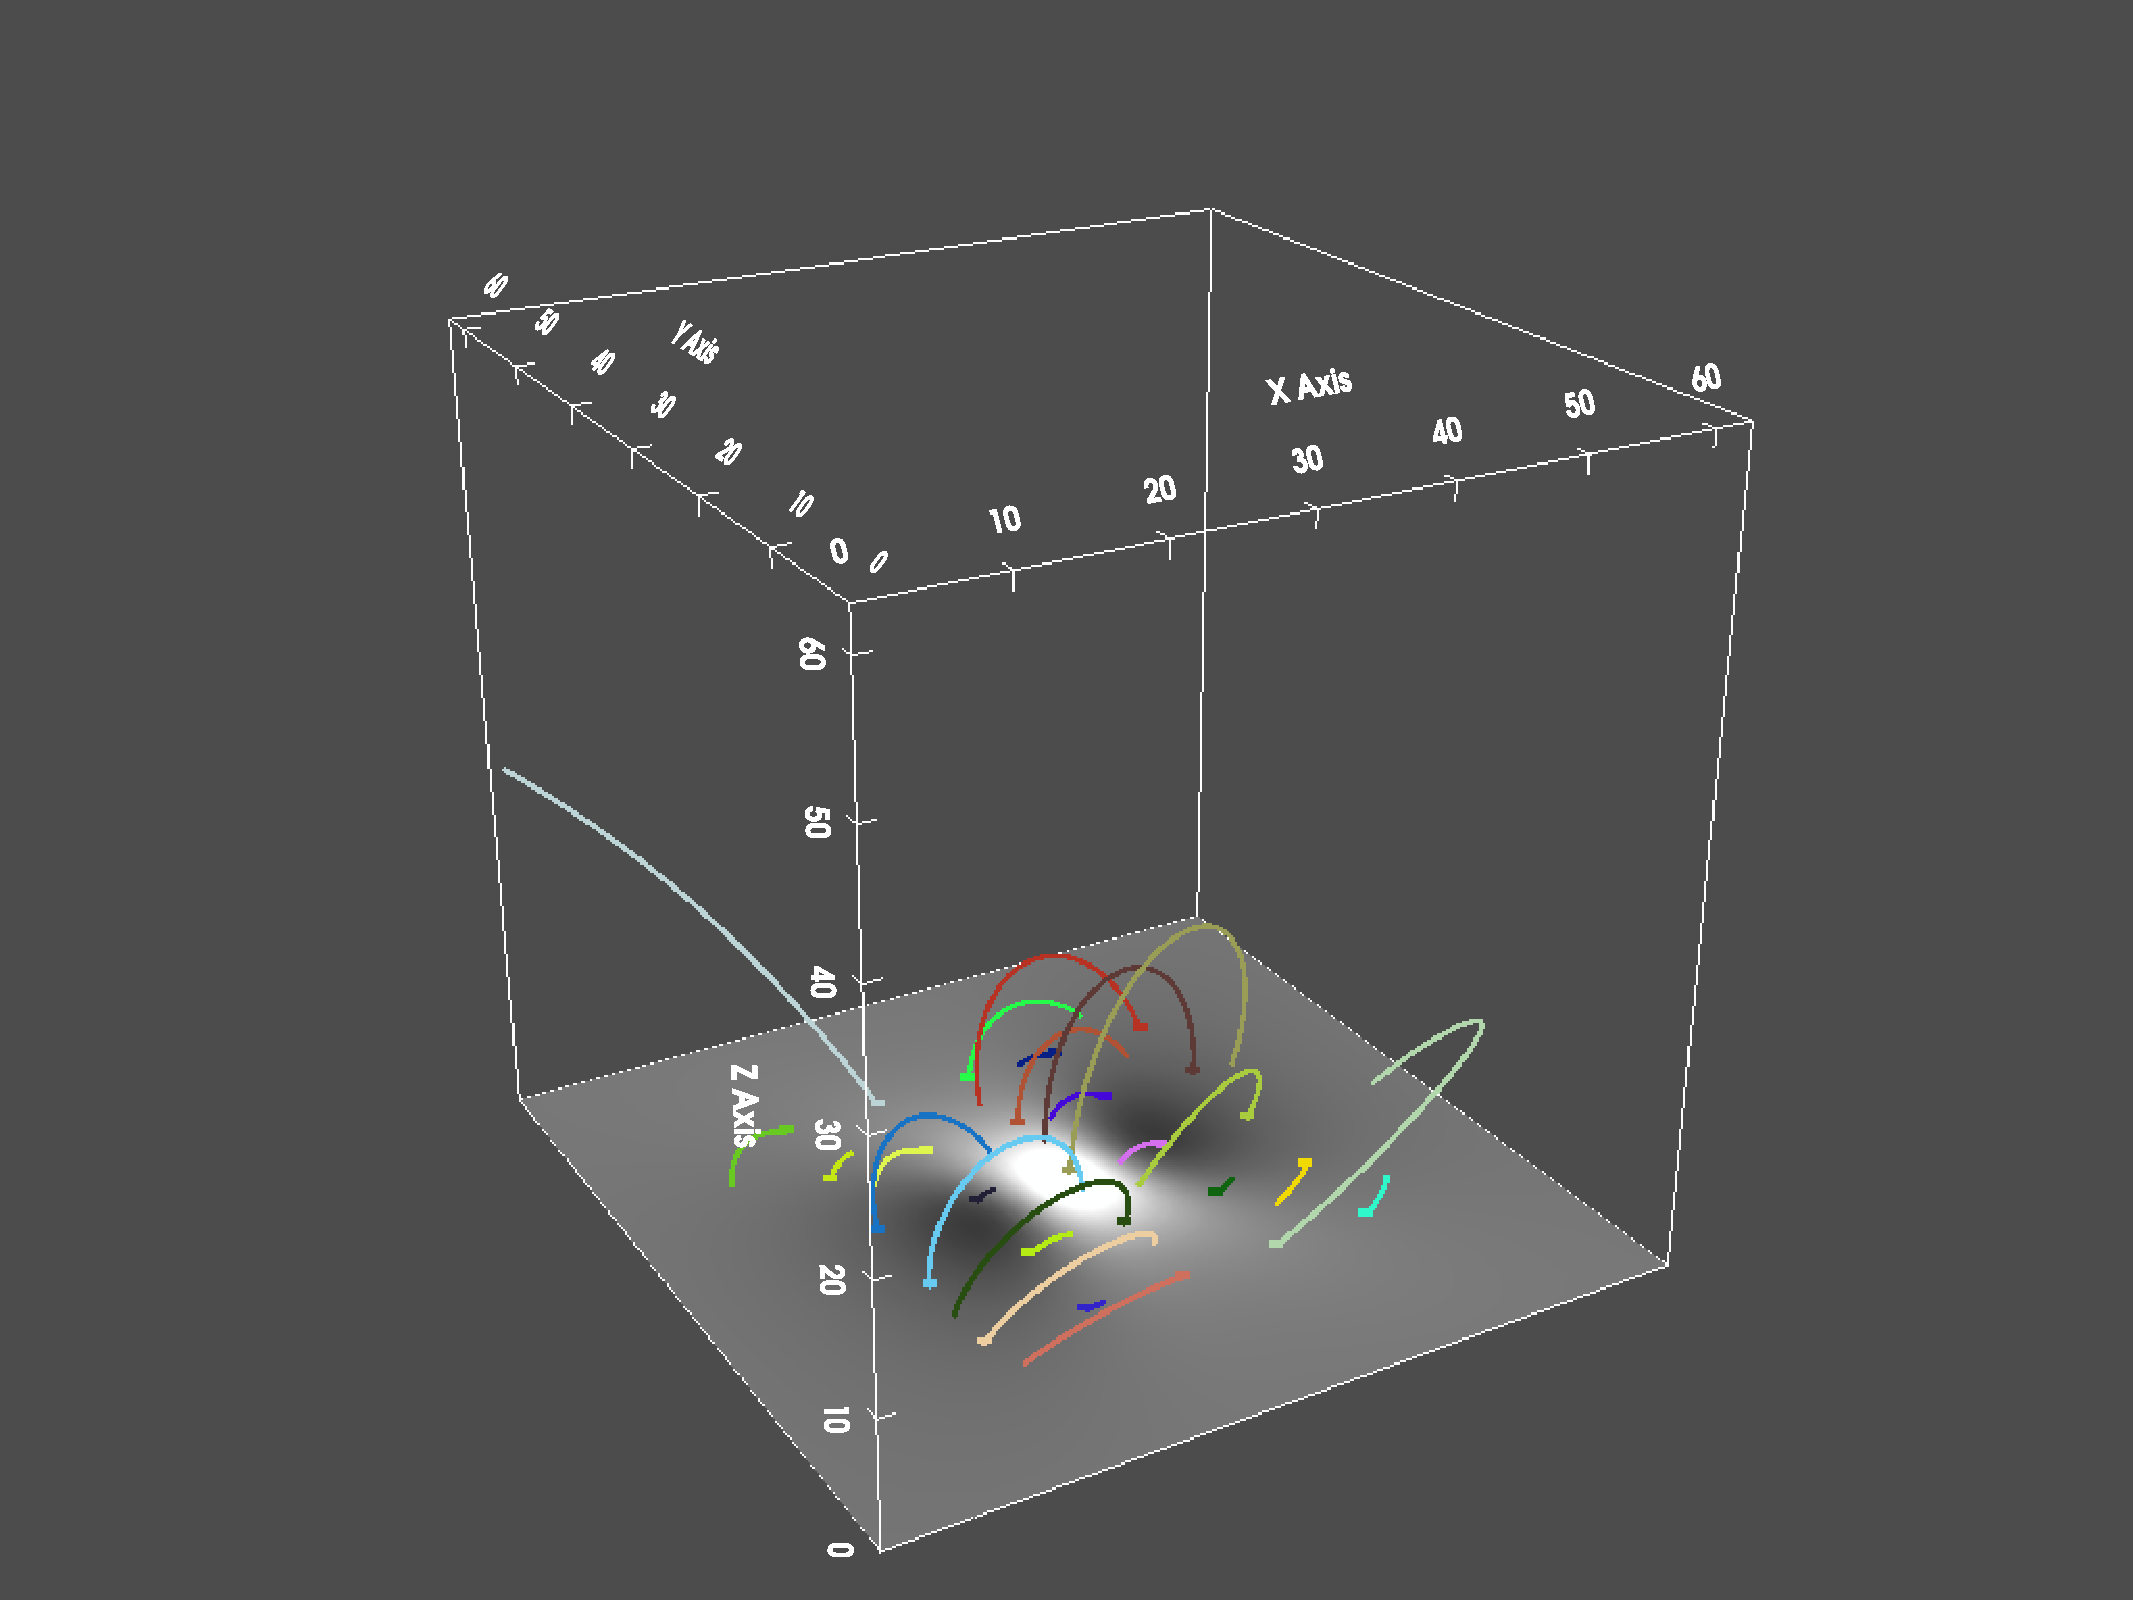
\includegraphics[trim={6cm 0cm 6cm 3cm}, clip, width=\linewidth]{"../../Thesis/img/LL_pot_xz_tilted.pdf"}
            \end{subfigure}%
            \begin{subfigure}{.5\linewidth}
              \centering
              \caption{\large Low-Lou}
              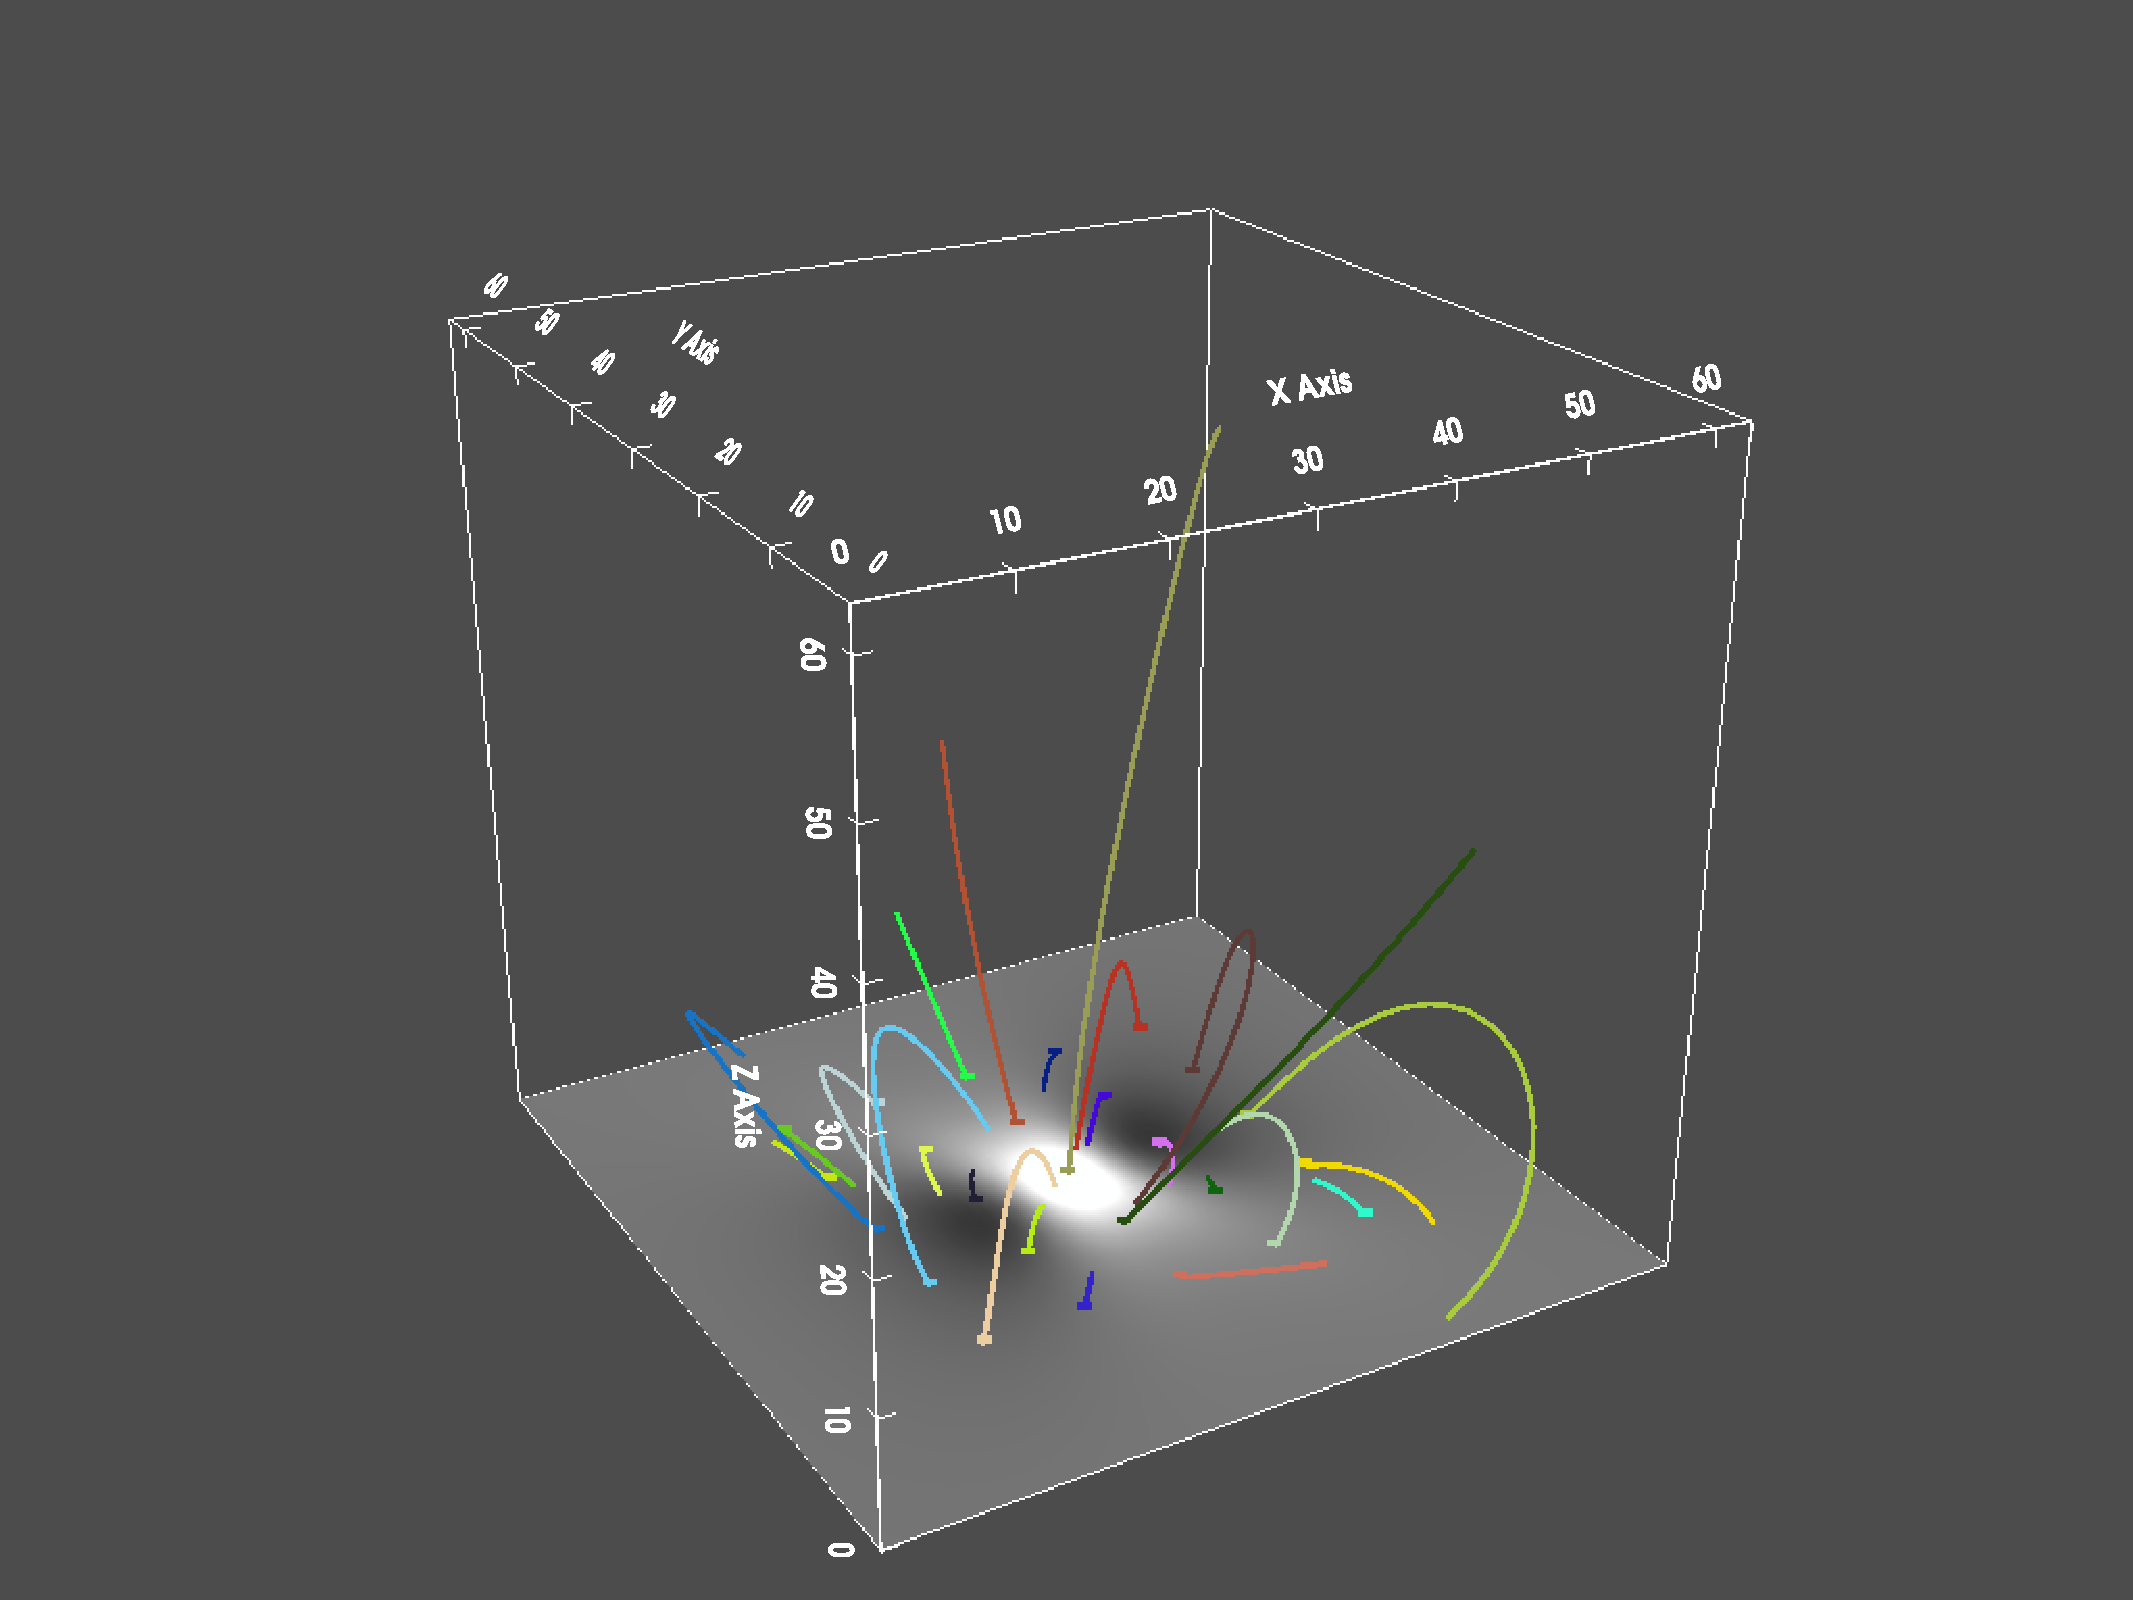
\includegraphics[trim={6cm 0cm 6cm 3cm}, clip, width=\linewidth]{"../../Thesis/img/LL_xz_tilted.pdf"}
            \end{subfigure}
            }
            
          \end{figure}
        \end{column}
    \end{columns}
  \end{frame}

  \begin{frame}{Loss}

    \begin{columns}
        \begin{column}{0.5\textwidth}
            \begin{figure}
                \begin{subfigure}{.5\linewidth}
                  \centering
                  \caption{$\mathcal{L}$}
                  \vspace*{-3mm}
                  \includegraphics[width=\linewidth]{"../../Thesis/img/graph/mathcal{L}_ylog.png"}
                  % \caption{The total loss of PINN.}
                \end{subfigure}%
                \begin{subfigure}{.5\linewidth}
                  \centering
                  \caption{$w_b\mathcal{L}_b$}
                  \vspace*{-3mm}
                  \includegraphics[width=\linewidth]{"../../Thesis/img/graph/w_bmathcal{L}_b_ylog.png"}
                  % \caption{The weighted loss of the boundary condition.}
                \end{subfigure}
              
                \begin{subfigure}{.5\linewidth}
                  \centering
                  \caption{$w_\text{ff}\mathcal{L}_\text{ff}$}
                  \vspace*{-3mm}
                  \includegraphics[width=\linewidth]{"../../Thesis/img/graph/w_text{ff}mathcal{L}_text{ff}_ylog.png"}
                  % \caption{The weighted loss of the force-free condition.}
                \end{subfigure}%
                \begin{subfigure}{.5\linewidth}
                  \centering
                  \caption{$w_\text{div}\mathcal{L}_\text{div}$}
                  \vspace*{-3mm}
                  \includegraphics[width=\linewidth]{"../../Thesis/img/graph/w_text{div}mathcal{L}_text{div}_ylog.png"}
                  % \caption{The weighted loss of the solenoidal condition.}
                \end{subfigure}
              \end{figure}
        \end{column}

        \begin{column}{0.5\textwidth}
            \begin{equation*}
                \mathbf{\hat{B}}=\mathcal{N}(\boldsymbol{x}; \boldsymbol{\theta})
            \end{equation*}
            \begin{align*}
                \mathcal{L}_\text{ff}(\boldsymbol{\theta}; \mathcal{T}_f) & = \frac{1}{|\mathcal{T}_f|} \sum_{\boldsymbol{x}\in \mathcal{T}_f} \frac{|(\nabla \times \mathbf{\hat{B}})\times \mathbf{\hat{B}}|^2}{|\mathbf{\hat{B}}|^2}\\
                \mathcal{L}_\text{div}(\boldsymbol{\theta}; \mathcal{T}_f) & = \frac{1}{|\mathcal{T}_f|} \sum_{\boldsymbol{x}\in \mathcal{T}_f} |\nabla \cdot \mathbf{\hat{B}}|^2\\
                \mathcal{L}_b(\boldsymbol{\theta};\mathcal{T}_b) & = \frac{1}{|\mathcal{T}_b|}\sum_{\boldsymbol{x}\in\mathcal{T}_b}{|\mathbf{\hat{B}}-\mathbf{B}|^2}\\
            \end{align*}
            \begin{equation*}
                \mathcal{L}_f = w_{\text{ff}}\mathcal{L}_\text{ff}+ w_{\text{div}}\mathcal{L}_\text{div} + w_b\mathcal{L}_b
            \end{equation*}
        \end{column}
        \end{columns}
  \end{frame}

  \begin{frame}{The 3D magnetic fields}
    \begin{columns}
      \begin{column}{0.9\textwidth}
      \begin{figure}
          \begin{subfigure}{.5\linewidth}
              \centering
              \caption{\large PINN(0)}
              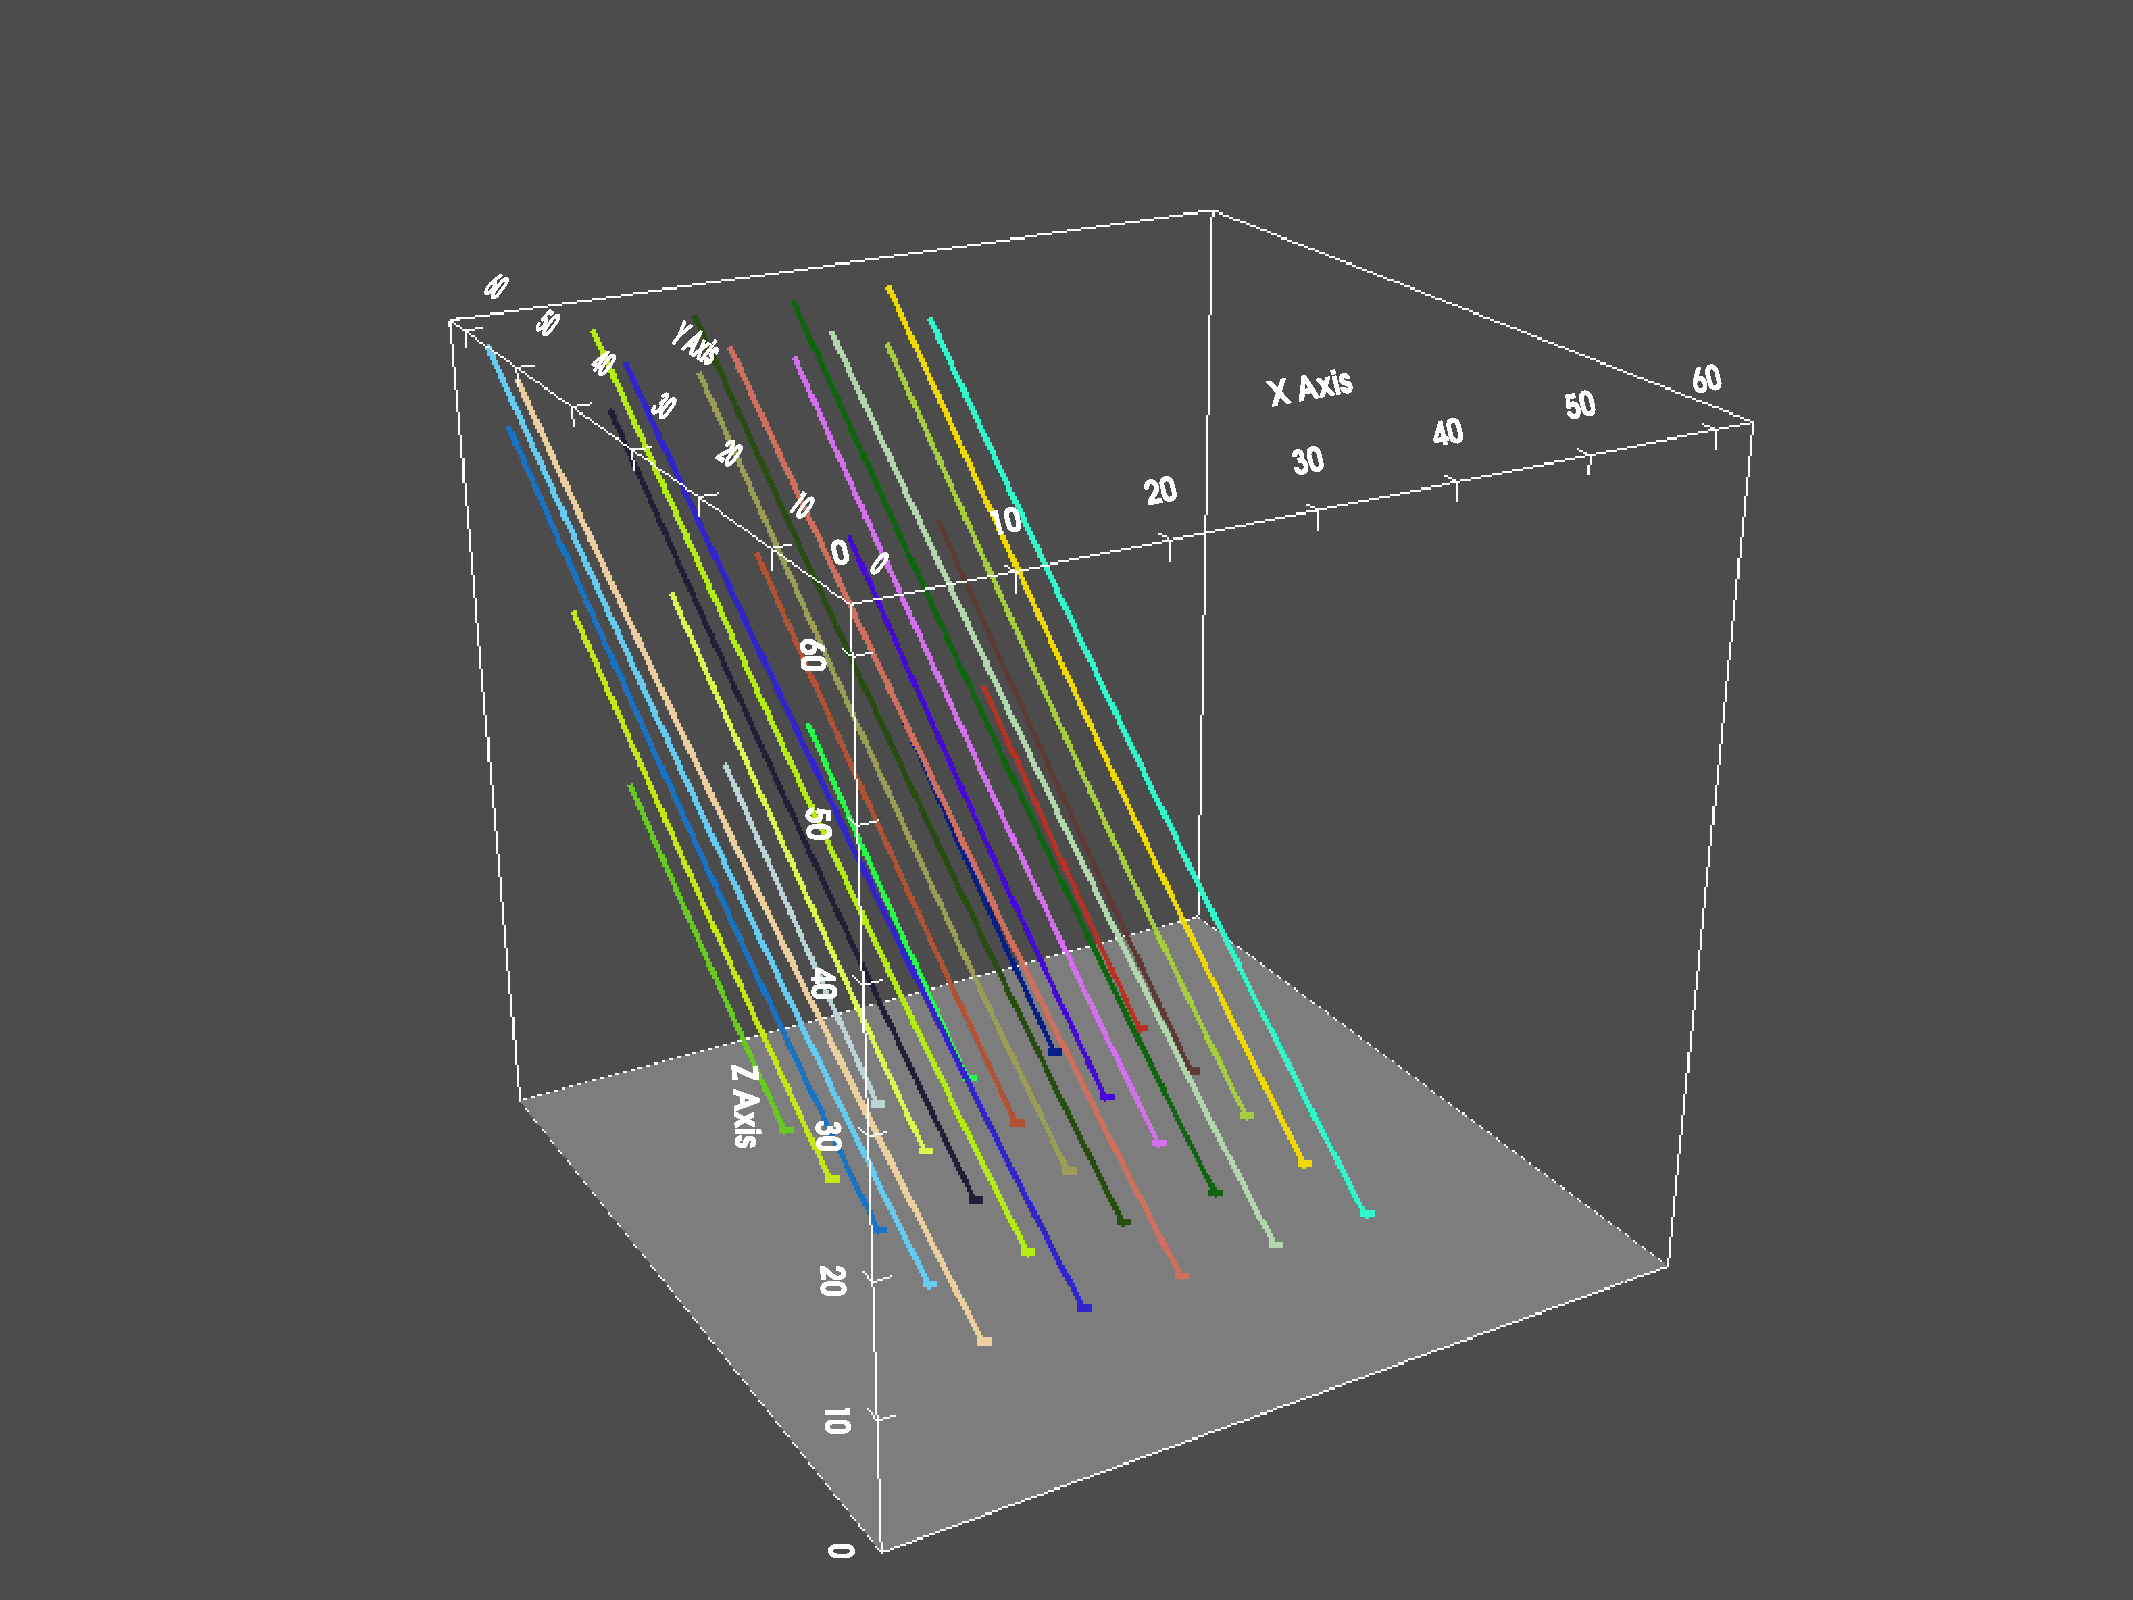
\includegraphics[trim={6cm 0cm 6cm 3cm}, clip, width=\linewidth]{"../../Thesis/img/PINN_000000_xz_tilted.pdf"}
            \end{subfigure}%
            \begin{subfigure}{.5\linewidth}
              \centering
              \caption{\large Low-Lou}
              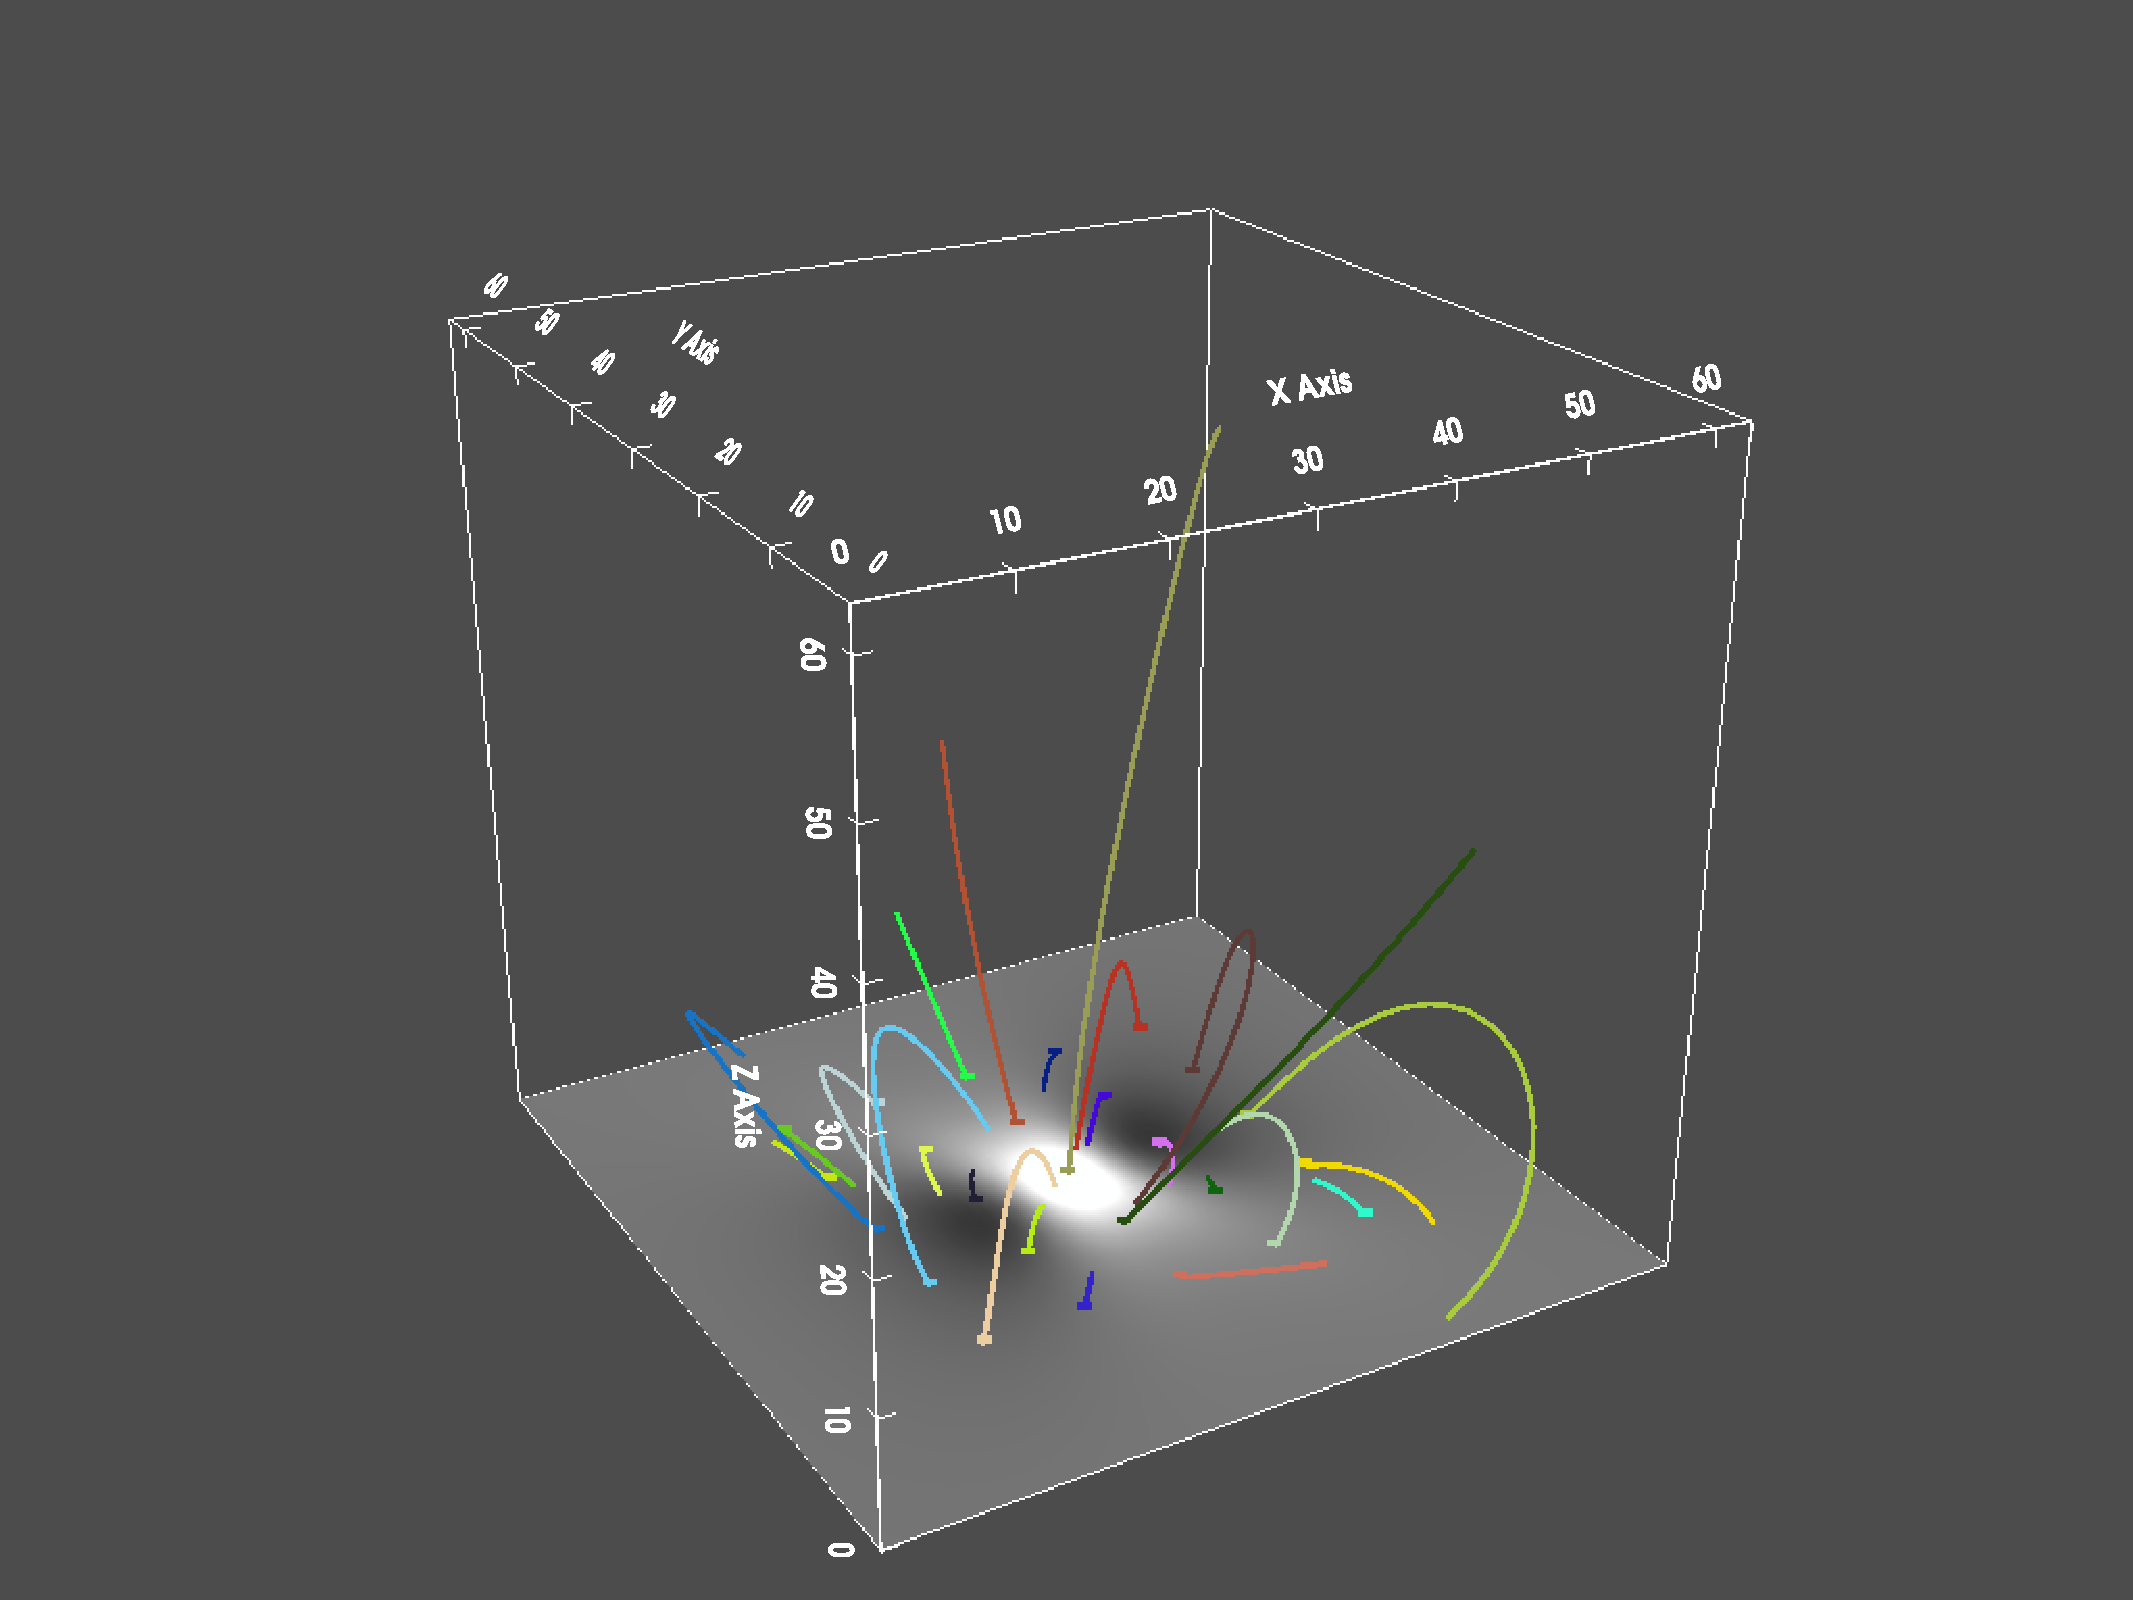
\includegraphics[trim={6cm 0cm 6cm 3cm}, clip, width=\linewidth]{"../../Thesis/img/LL_xz_tilted.pdf"}
            \end{subfigure}
        \end{figure}
      \end{column}
  \end{columns}
  \end{frame}

  \begin{frame}{Figures of merit \parencite{schrijver2006nonlinear}}

    \begin{columns}
        \begin{column}{0.5\textwidth}
            \begin{align*}
                C_\text{vec} & = \frac{\sum_i \mathbf{B}_i \cdot \mathbf{b}_i}{(\sum_i |\mathbf{B}_i|^2 \sum_i |\mathbf{b}_i|^2)^{1/2}} \\
                C_\text{CS} & = \frac{1}{M} \sum_i \frac{\mathbf{B}_i \cdot \mathbf{b}_i}{|\mathbf{B}_i||\mathbf{b}_i|}\\
                E'_n & = 1 - \frac{\sum_i |\mathbf{B}_i - \mathbf{b}_i|}{\sum_i |\mathbf{b}_i|}\\
                E'_m & = 1 - \frac{1}{M} \frac{\sum_i |\mathbf{B}_i - \mathbf{b}_i|}{\sum_i |\mathbf{b}_i|}\\
            \end{align*}
        \end{column}
        \begin{column}{0.5\textwidth}  %%<--- here

            \begin{align*}
                \epsilon & = \frac{\sum_i |\mathbf{B}_i|^2}{\sum_i |\mathbf{b}_i|^2}\\
                \epsilon_p & = \frac{\sum_i |\mathbf{B}_i|^2}{\sum_i |\mathbf{B}_{\text{p}, i}|^2} \\
                \text{CW}_\text{sin} & = \frac{\sum_i \frac{|\mathbf{J}_i \times \mathbf{B}_i|}{|\mathbf{B}_i|}}{\sum_i |\mathbf{J}_i|}
            \end{align*}
            
        \end{column}
        \end{columns}
        Here, $i$ refers to each grid point, $M$ is the total number of grid points, $\mathbf{B}$ is the numerical magnetic field, $\mathbf{b}$ is the reference magnetic field, $\mathbf{B}_{\text{p}}$ is the potential magnetic field whose bottom boundary condition is the same as that of $\mathbf{B}$, and $\mathbf{J} = \nabla \times \mathbf{B}$ is the current density in an appropriate unit system.
  \end{frame}

  \begin{frame}{Figures of merit + Loss}
    \begin{columns}
        \begin{column}{\textwidth}
        \begin{figure}
            \begin{subfigure}{0.25\linewidth}
            \centering
            \caption{$C_\text{vec}$}
            \vspace*{-3mm}
            \includegraphics[width=\linewidth]{"../../Thesis/img/graph/C_{text{vec}}.png"}
            % \caption{The total loss of PINN.}
            \end{subfigure}%
            \begin{subfigure}{0.25\linewidth}
            \centering
            \caption{$C_\text{CS}$}
            \vspace*{-3mm}
            \includegraphics[width=\linewidth]{"../../Thesis/img/graph/C_{text{CS}}.png"}
            % \caption{The weighted loss of the boundary condition.}
            \end{subfigure}%
            \begin{subfigure}{0.25\linewidth}
            \centering
            \caption{$E'_n$}
            \vspace*{-3mm}
            \includegraphics[width=\linewidth]{"../../Thesis/img/graph/E^{prime}_{n}.png"}
            % \caption{The weighted loss of the force-free condition.}
            \end{subfigure}%
            \begin{subfigure}{0.25\linewidth}
            \centering
            \caption{$E'_m$}
            \vspace*{-3mm}
            \includegraphics[width=\linewidth]{"../../Thesis/img/graph/E^{prime}_{m}.png"}
            % \caption{The weighted loss of the solenoidal condition.}
            \end{subfigure}

                \begin{subfigure}{0.25\linewidth}
                \centering
                \caption{$\epsilon$}
                \vspace*{-3mm}
                \includegraphics[width=\linewidth]{"../../Thesis/img/graph/epsilon_ylog.png"}
                % \caption{The weighted loss of the force-free condition.}
                \end{subfigure}%
                \begin{subfigure}{0.25\linewidth}
                \centering
                \caption{$\epsilon_p$}
                \vspace*{-3mm}
                \includegraphics[width=\linewidth]{"../../Thesis/img/graph/epsilon_p_ylog.png"}
                % \caption{The weighted loss of the solenoidal condition.}
                \end{subfigure}%
                \begin{subfigure}{0.25\linewidth}
                \centering
                \caption{$\text{CW}_\text{sin}$}
                \vspace*{-3mm}
                \includegraphics[width=\linewidth]{"../../Thesis/img/graph/CW_{text{sin}}.png"}
                % \caption{The weighted loss of the force-free condition.}
                \end{subfigure}%
                \begin{subfigure}{0.25\linewidth}
                \centering
                \caption{$\mathcal{L}$}
                \vspace*{-3mm}
                \includegraphics[width=\linewidth]{"../../Thesis/img/graph/mathcal{L}_ylog.png"}
                % \caption{The weighted loss of the solenoidal condition.}
                \end{subfigure}
              \end{figure}
            \end{column}
        \end{columns}
  \end{frame}

  \begin{frame}{Figures of merit + Loss}
        
    \resizebox{\textwidth}{!}{%
    \begin{NiceTabular}{ccccccccc}
        \toprule
        Field & $C_\text{vec}$ & $C_\text{CS}$ & $E'_n$ & $E'_m$ & $\epsilon$ & $\epsilon_p$ & $\text{CW}_\text{sin}$ & $\mathcal{L}$\footnote{The total loss of PINN.} \\ 
        \midrule
        Low-Lou\footnote{The parameters of the Low-Lou model are $(n=1, m=1, l=0.3, \Phi=\pi/2)$.} & 1.00000 & 1.00000 & 1.00000 & 1.00000 & 1.00000 & 1.44490 & 0.01308\footnote{This is not zero due to numerical grids.} & -- \\
        Potential & 0.86465 & 0.86925 & 0.43003 & 0.36242 & 0.69209 & 1.00000 & --\footnote{The metric $\text{CW}_\text{sin}$ is undefined for the potential field.} & -- \\
        PINN(0) & 0.07115 & 0.33540 & -1.37088 & -6.07067 & 0.71824 & 1.03779 & 0.55813 & 40.23570 \\
        PINN(100) & 0.25771 & 0.46100 & -0.00643 & -0.46701 & 0.08056 & 0.11640 & 0.76066 & 31.32017 \\
        PINN(1000) & 0.54244 & 0.32404 & -2.31914 & -6.41640 & 5.59377 & 8.08246 & 0.71701 & 6.46577 \\
        PINN(10000) & 0.98630 & 0.63065 & 0.68766 & 0.28275 & 0.96939 & 1.40068 & 0.38403 & 0.00848 \\
        PINN(25000) & 0.99402 & 0.92134 & 0.78452 & 0.55897 & 0.96481 & 1.39406 & 0.07853 & 0.00006 \\
        PINN(50000) & 0.99359 & 0.92271 & 0.77129 & 0.50928 & 0.96247 & 1.39068 & 0.06848 & 0.00005 \\
        \bottomrule
        \end{NiceTabular}
  }
  \end{frame}

\end{document}